
% LATEX version of the PETSc developers manual.
%

% A common preamble shared between the dev manual and the manual
% Common preamble used by the manuals
\documentclass[twoside,11pt]{../sty/report_petsc}

\usepackage{fixltx2e}
\usepackage{makeidx,xspace}
\usepackage[bookmarksopen,colorlinks]{hyperref}
\usepackage[all]{hypcap}
\usepackage{xcolor}
\input pdfcolor.tex

\usepackage[pdftex]{graphicx}

%\usepackage{times}
\usepackage{tikz}
\usepackage{../sty/verbatim}
\usepackage{../sty/tpage}
\usepackage{../sty/here}
\usepackage{../sty/anlhelper}

% At the time of this writing, only used for \text{} in math mode
\usepackage{amsmath}

% trl is used to refer to URLs, command line arguments, paths, and other "mentions"
%\usepackage[obeyspaces]{../sty/trl}
\usepackage[hyphens,spaces,obeyspaces]{../sty/trl}

% Listings are used to refer to literal code
\usepackage{listings}
\usepackage{xcolor}
\definecolor{verylightgray}{gray}{0.95}
\definecolor{somewhatdarkgray}{gray}{0.3}

% General/default listing settings are for C code

% Note : $ (not used in C) is an escape character,
% so using this for languages that include this will give some 
% strange errors as you escape to LaTeX

% Note : When using \lstinline inside a table,
% use pipes as delimiters, like \lstinline|VecCopy()|
% This is hardcoded into lib/petsc/bin/maint/mapnameslatex.py
\lstset{
  language=C,
  basicstyle=\normalsize\ttfamily,
  escapechar=\$,        % Also hardcoded in lib/petsc/bin/maint/mapnameslatex.py
  commentstyle=\color{somewhatdarkgray}\ttfamily,
  showstringspaces=false,
  basewidth=0.5em,      % For consistent spacing with inline listings
  breaklines=true,
  backgroundcolor=\color{verylightgray},
  frame=single,
  framexleftmargin= 3px,
  framexrightmargin= 3px,
  rulecolor=\color{lightgray},
  breakatwhitespace=true,
}

% Some special listing environments for various code types
% We could consider using a dedicated clisting (but be careful with the inline listings)

\lstnewenvironment{outputlisting}[1][\footnotesize\ttfamily]
{\lstset{escapechar=,language=,basicstyle=#1,breakatwhitespace=false}}
{}

\lstnewenvironment{bashlisting}
{\lstset{escapechar=,language=bash,basicstyle=\ttfamily}}
{}

\lstnewenvironment{makelisting}
{\lstset{escapechar=,language=make,basicstyle=\ttfamily}}
{}

% Set all nested itemize labels to be the same
\renewcommand{\labelitemi}{$\bullet$}
\renewcommand{\labelitemii}{$\bullet$}
\renewcommand{\labelitemiii}{$\bullet$}
\renewcommand{\labelitemiv}{$\bullet$}

% Define a tighter itemize and enumerate
% To be used when all entries are a single line.
\newenvironment{tightitemize}
{ \begin{itemize}
  \setlength{\itemsep}{1pt}
  \setlength{\parskip}{1pt}
  \setlength{\parsep}{1pt} }
{ \end{itemize} } 
\newenvironment{tightenumerate}
{ \begin{enumerate}
  \setlength{\itemsep}{1pt}
  \setlength{\parskip}{1pt}
  \setlength{\parsep}{1pt} }
{ \end{enumerate} } 

\setlength{\textwidth}{6.5in}
\setlength{\oddsidemargin}{0.0in}
\setlength{\evensidemargin}{0.0in}
\setlength{\textheight}{9.2in}
\setlength{\topmargin}{-.8in}

\newcommand{\findex}[1]{\index{#1}}
\newcommand{\sindex}[1]{\index{#1}}
\newcommand{\A}{\mbox{\boldmath \(A\)}}
\newcommand{\F}{\mbox{\boldmath \(F\)}}
\newcommand{\J}{\mbox{\boldmath \(J\)}}
\newcommand{\x}{\mbox{\boldmath \(x\)}}
\newcommand{\bb}{\mbox{\boldmath \(b\)}}
\newcommand{\rr}{\mbox{\boldmath \(r\)}}

\usepackage{fancyhdr,lastpage}


\def\shortintro{false}

\usepackage{fancyhdr,lastpage}
\pagestyle{fancy}
\rhead{PETSc 3.10 \today}

\begin{document}

\pagestyle{empty}
\hspace{-.65in}
\includegraphics{ArgonneLogo}
\hfill  {\large {\bf ANL-18/18 Rev 3.10}}

\vspace*{2in}
\noindent {\huge{\bf PETSc Developers Guide}}
\vspace*{8pt}
\hrule
\vspace*{8pt}
\noindent {\Large{\it Revision 3.10}}

\vspace*{1in}
\noindent \\
{\Large {\bf Mathematics and Computer Science Division}}

\vspace*{10pt}
\vspace*{20pt}


%%%%%%%%%%%%%%%%%%%%%%%%%%%%%%%%%%%%%%%%%%%%%%%%%%%%%%%%%%%%%%%%%%%%%%%%%%%%%%%%%%%%

\newpage
\centerline{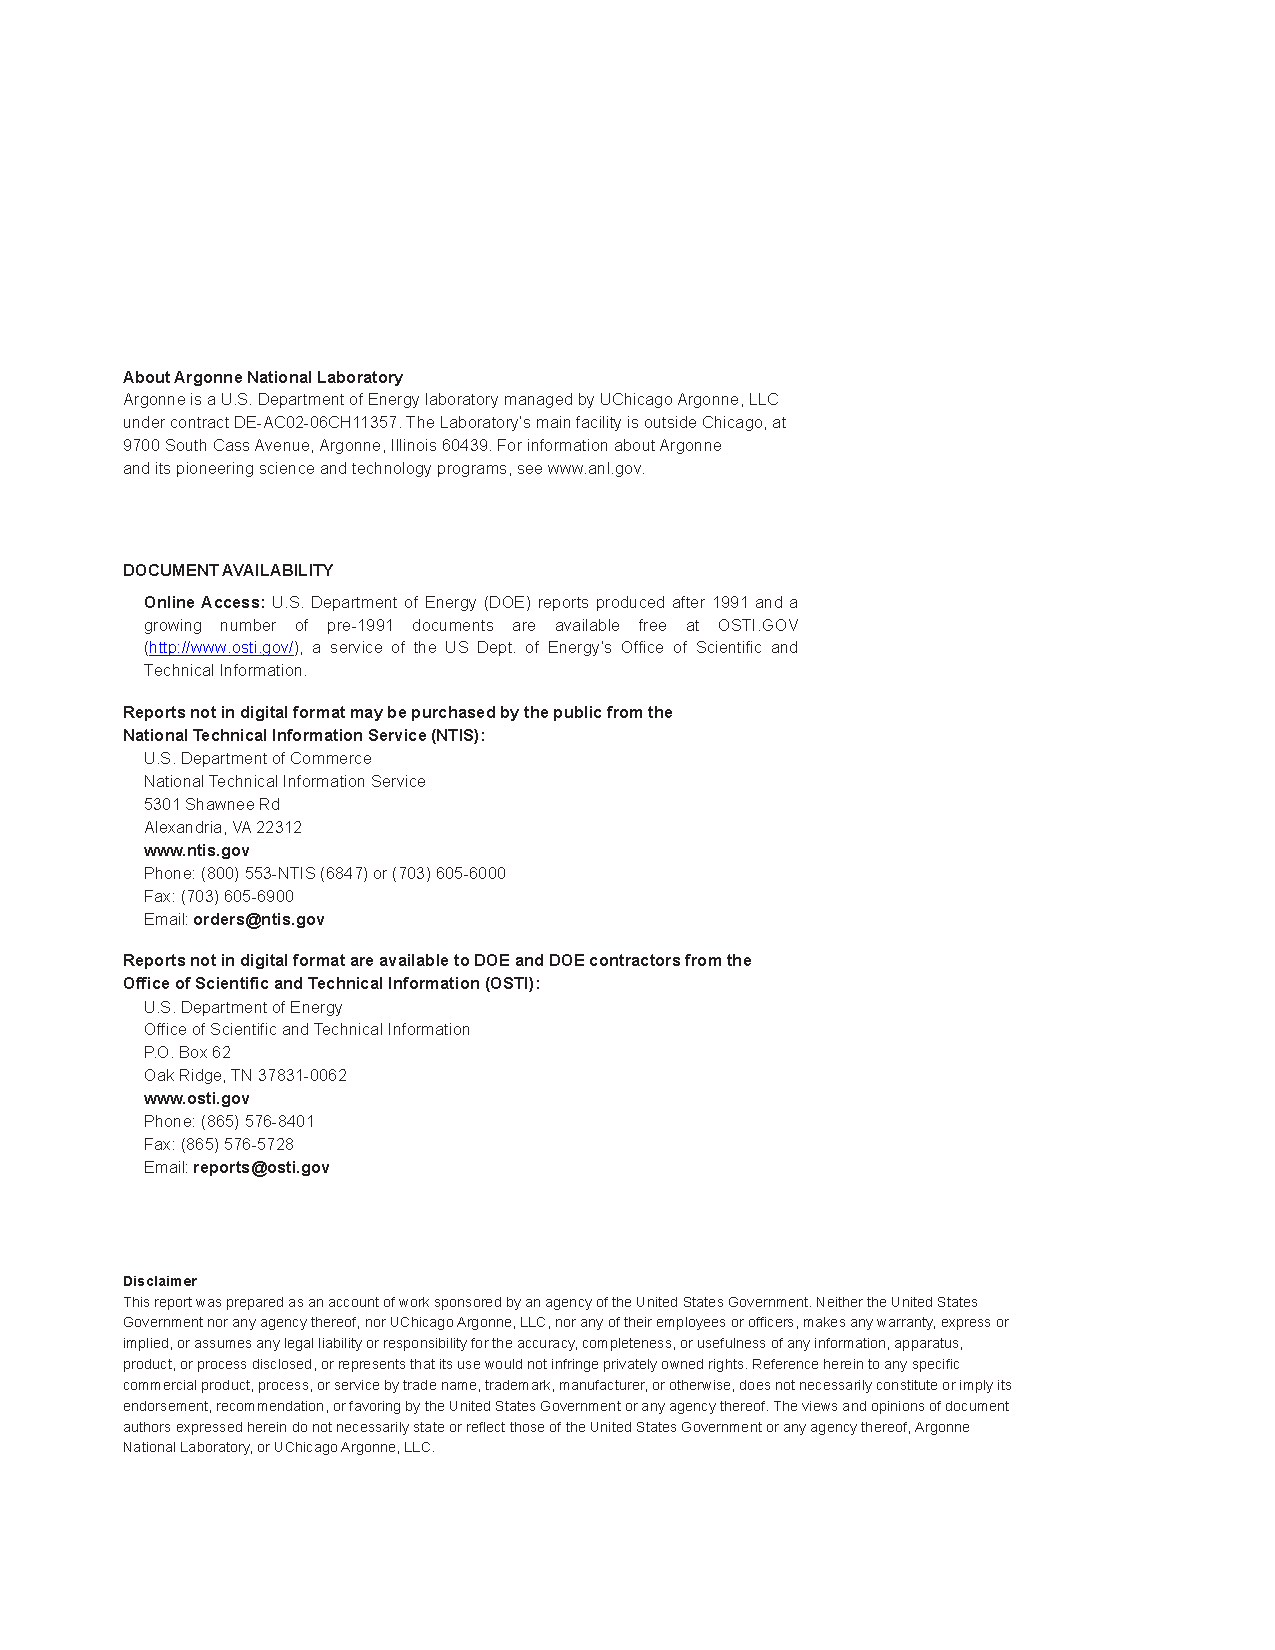
\includegraphics{ArgonneReportTemplate2018Page2}}
\newpage

\hfill {\large {\bf ANL-18/18 Rev 3.10}}

\vspace*{2in}
\noindent {\LARGE{\bf PETSc Developers Manual}}
\vspace*{8pt}
\hrule
\vspace*{8pt}
\noindent {\Large{\it Revision 3.10}}

\vspace*{0.5in}
\noindent Prepared by \\
{S. Kruger\textsuperscript{1}, P. Sanan\textsuperscript{2}, and B. Smith\textsuperscript{3}}\\
\\
\textsuperscript{1}Tech-X Corporation \\
\textsuperscript{2}Institute of Geophysics, ETH Zurich\\
\textsuperscript{3}Mathematics and Computer Science Division, Argonne National Laboratory \\

\vspace*{30pt}
\noindent June 2018

\vspace*{20pt}
\noindent This material was based upon work supported by the Office of Science, Office of Advanced Scientific Computing Research, \\
U.S. Department of Energy, under Contract DE-AC02-06CH11357.


\newpage

\hbox{ }

\vspace{1in}
\date{\today}

% Blank page makes double sided printout look bettter.
\pagestyle{empty}
\newpage

\medskip \medskip

%
%   Next line temp removed
%
\noindent {\bf Abstract}

\medskip \medskip
PETSc is an extensible software library for scientific
computation. This document provides information for PETSc
developers and those wishing to contribute to PETSc. The text assumes
that you are familiar with PETSc and have access to PETSc source code
and documentation (available
via \href{http://www.mcs.anl.gov/petsc}{http://www.mcs.anl.gov/petsc}) including the PETSc users manual \cite{petsc-user-ref}.
Higher-level views of PETSc can be found in \cite{s2011}, \cite{bgms00}, \cite{miss-paper}, \cite{bgms98}, and \cite{petsc-efficient}. 

Before contributing code to PETSc, please read Chapter \ref{chapter:styleguide}, which contains the source code style guide.
Information on how to submit patches and pull requests to PETSc can be found at
\href{http://www.mcs.anl.gov/petsc/developers/index.html}{http://www.mcs.anl.gov/petsc/developers/index.html}.

\vspace{1cm}

Please direct all comments and questions regarding PETSc design and
development to \trl{petsc-dev@mcs.anl.gov}.  Note that all {\em
bug reports and questions regarding the use of PETSc} should
be directed to \trl{petsc-maint@mcs.anl.gov}.

%
% NOTES:
%  - Be sure to place captions BEFORE labels in figures and tables!
%    Otherwise, numbering will be incorrect.  For example, use the following:
%       \caption{PETSc Vector Operations}
%       \label{fig:vectorops}
%  - Use \break to indicate a line break (needed to prevent long strings in
%    \tt mode from running of the page)
%

% Blank page makes double sided printout look bettter.
\newpage
\hbox{ }
\newpage

\tableofcontents

\pagestyle{fancy}
\chapter{Responding to User Requests and Questions}

PETSc users communicate to the PETSc team via two mailing lists:
petsc-maint@mcs.anl.gov and petsc-users@mcs.anl.gov. When responding
to such inquiries, please follow the guidelines given below.

\begin{tightitemize}
\item Be polite.
\item Address the person by name (when you can determine the name).
\item Apologize for the problem when it is appropriate (but not otherwise).
\item Thank the person for his or her patience if it is more than six hours since the report came in.
\item If the person drops the \trl{petsc-maint} or \trl{petsc-users} from the reply list, add it back in.
\item Don't ask too many questions or give too many suggestions in the same email. The user often responds only to the first of them or becomes confused.
\end{tightitemize}

\chapter{Style Guide}\label{chapter:styleguide}

The PETSc team uses certain conventions to make the source code consistent and hence easier to maintain. We will interchangeably use the
terminology {\em subclass}, {\em implementation}, or {\em type}\footnote{Type also refers to the string name of the subclass.}
to refer to a concrete realization of an abstract base class. For example, \lstinline{KSPGMRES} is a type for the base class \lstinline{KSP}.

\section{Names}\label{sec:stylenames}
Consistency of names for variables, functions, and so on is extremely
important.
We use several conventions
\begin{enumerate}
\item All function names and enum types consist of acronyms or words, each of
  which is capitalized, for example, \lstinline{KSPSolve()} and
      \lstinline{MatGetOrdering()}.
\item All enum elements and macro variables are named with all capital letters. When
      they consist of several complete words, there is an underscore between each word.
      For example, \lstinline{MAT_FINAL_ASSEMBLY}.
\item Functions that are private to PETSc (not callable by the
      application code) either
      \begin{itemize}
        \item have an appended \lstinline{_Private} (for example,
           \lstinline{StashValues_Private}) or
        \item have an appended \lstinline{_Subtype} (for example,
           \lstinline{MatMult_SeqAIJ}).
      \end{itemize}

      In addition, functions that are not intended for use outside
      of a particular file are declared \lstinline{static}.
      Also see item \ref{styleitem:petscextern} in Section \ref{sec:stylepetsc}.
\item Function names in structures (for example, \lstinline{_matops}) are the same as the base application
      function name without the object prefix and are in small letters.
      For example, \lstinline{MatMultTranspose()} has a structure name of
      \lstinline{multtranspose}.
\item Names of implementations of class functions should begin with the function name, an underscore, and the name of the implementation, for example, \lstinline{KSPSolve_GMRES()}.
\item Each application-usable function begins with the name of the class object, followed by any subclass name,
  for example, \lstinline{ISInvertPermutation()}, \lstinline{MatMult()}, or \lstinline{KSPGMRESSetRestart()}.
\item Functions that PETSc provides as defaults for user-providable functions end with \lstinline{Default} (for example, \lstinline{KSPMonitorDefault()} or \lstinline{PetscSignalHandlerDefault()}).
\item Options database keys are lower case, have an underscore between words, and match the function name associated with the option without the word ``set'' or ``get'',
for example, \trl{-ksp_gmres_restart}.
\item Specific \lstinline{XXXType} values (for example, \lstinline{MATSEQAIJ}) do not have an underscore in them unless they refer to another package that uses an underscore, for example, \lstinline{MATSOLVERSUPERLU_DIST}.
\end{enumerate}

\section{Coding Conventions and Style}
Within the PETSc source code, we adhere to the following guidelines
so that the code is uniform and easily maintained.

\subsection{C Formatting}
\begin{enumerate}
\item {\em No} tabs are allowed in {\em any} of the source code.
\item All PETSc function bodies are indented two characters.
\item Each additional level of loops, \lstinline{if} statements, and so on is indented
      two more characters.
\item Wrapping lines should be avoided whenever possible.
\item Source code lines do not have a hard length limit; generally, we like them less than 150 characters wide.
\item The local variable declarations should be aligned. For example,
      use the style
\begin{lstlisting}
PetscScalar a;
PetscInt    i,j;
\end{lstlisting}
instead of
\begin{lstlisting}
PetscScalar a;
PetscInt i,j; /* Incorrect */
\end{lstlisting}

\item Assignment and comparison operations, for example, \lstinline{x = 22.0} or
\lstinline{x < 22.0}, should have single spaces around the operator.
This convention is true even when assignments are given directly in a line that declares
the variable, such as \lstinline{PetscReal r = 22.3}. The exception is when
these symbols are used in a \lstinline{for} loop; then, there should be no spaces,
for example, \lstinline{for (i=0; i<m; i++)}. Comparisons in \lstinline{while()}
constructs should have the spaces.
\item When declaring variables there should be no space between multiple variables, for example, \lstinline{PetscReal a,b,c}, not \lstinline{PetscReal a, b, c}.
\item The prototypes for functions should not include the names of the variables; for example, write
\begin{lstlisting}
PETSC_EXTERN PetscErrorCode MyFunction(PetscInt);
\end{lstlisting}
not
\begin{lstlisting}
PETSC_EXTERN PetscErrorCode MyFunction(PetscInt myvalue); /* Incorrect */
\end{lstlisting}
\item All local variables of a particular type (for example, \lstinline{PetscInt}) should be
      listed on the same line if possible; otherwise, they should be listed
      on adjacent lines.
\item Equal signs should be aligned in regions where possible.
\item There {\em must} be a single blank line
      between the local variable declarations and the body of the function.
\item Indentation for \lstinline{if} statements {\em must}  be done  as follows.
\begin{lstlisting}
if ( ) {
  ....
} else {
  ....
}
\end{lstlisting}
\item {\em Never} have
\begin{lstlisting}
if ( )
  a single indented line /* Incorrect */
\end{lstlisting}
or
\begin{lstlisting}
for ( )
  a single indented line /* Incorrect */
\end{lstlisting}
Instead, use either
\begin{lstlisting}
if ( ) a single statement
\end{lstlisting}
or
\begin{lstlisting}
if ( ) {
  a single indented line
}
\end{lstlisting}
Note that error checking is a separate statement, so the following is {\em incorrect}
\begin{lstlisting}
if ( ) ierr = XXX();CHKERRQ(ierr); /* Incorrect */
\end{lstlisting}
and instead you should use
\begin{lstlisting}
if ( ) {
  ierr = XXX();CHKERRQ(ierr);
}
\end{lstlisting}
\item Always have a space between \lstinline{if} or \lstinline{for} and the following \lstinline{()}.
\item \label{styleitem:bracesameline} The open brace should be on the same line as the \lstinline{if ( )} test, \lstinline{for ( )}, and so forth, not on its own line, for example,
\begin{lstlisting}
 } else {
\end{lstlisting}
instead of
\begin{lstlisting}
 }
 else { /* Incorrect */
\end{lstlisting}
See item \ref{styleitem:bracenextline} for an exception.
 The closing brace should {\em always} be on its own line.
\item \label{styleitem:bracenextline} In function declarations, the opening brace should be on the {\em next} line, not on the same line as the function name and arguments.
  This is an exception to item \ref{styleitem:bracesameline}.
\item Do not leave sections of commented-out code in the source files.
\item Do not use C++-style comments (\lstinline{// Comment}). Use only C-style comments (\lstinline{/* Comment */}).
\item All variables must be declared at the beginning of the code block (C89 style), never mixed in with code.
\item Do not include a space after a \lstinline{(} or before a \lstinline{)}. Do not write
\begin{lstlisting}
ierr = PetscMalloc1( 10,&a );CHKERRQ(ierr); /* Incorrect */
\end{lstlisting}
but instead write
\begin{lstlisting}
ierr = PetscMalloc1(10,&a);CHKERRQ(ierr);
\end{lstlisting}
\item Do not use a space after the \lstinline{)} in a cast or between the type and the \lstinline{*} in a cast.
\item Do not include a  space before or after a comma in lists.
That is, do not write
\begin{lstlisting}
ierr = func(a, 22.0);CHKERRQ(ierr); /* Incorrect */
\end{lstlisting}
but instead write
\begin{lstlisting}
ierr = func(a,22.0);CHKERRQ(ierr);
\end{lstlisting}
\end{enumerate}


\subsection{C Usage}
\begin{enumerate}
\item Array and pointer arguments where the array values are not changed should be labeled as \lstinline{const} arguments.
\item Scalar values passed to functions should {\em never} be labeled as \lstinline{const}.
\item Subroutines that would normally have a \lstinline{void**} argument to return a pointer to some data should
actually be prototyped as \lstinline{void*}. This prevents the caller from having to put a \lstinline{(void**)} cast in each function call. See, for example, \lstinline{DMDAVecGetArray()}.
\item Do not use the \lstinline{register} directive.
\item Do not use \lstinline{if (rank == 0)} or \lstinline{if (v == NULL)} or \lstinline{if (flg == PETSC_TRUE)} or \lstinline{if (flg == PETSC_FALSE)}.
Instead, use \lstinline{if (!rank)} or \lstinline{if (!v)} or \lstinline{if (flg)} or \lstinline{if (!flg)}.
\item Do not use \lstinline{#ifdef} or \lstinline{#ifndef}. Rather, use \lstinline{#if defined(...} or \lstinline{#if !defined(...}
\item Never use system random number generators such as \lstinline{rand()} in PETSc code or examples because these can produce different results
on different systems thus making portability testing difficult. Instead use \lstinline{PetscRandom} which produces the exact same results regardless of
system it is used on.
\end{enumerate}

\subsection{Usage of PETSc Functions and Macros}
\label{sec:stylepetsc}
\begin{enumerate}
\item Public PETSc include files, \trl{petsc*.h}, should not reference private PETSc \trl{petsc/private/*impl.h} include files.
\item Public and private PETSc include files cannot reference include files located in the PETSc source tree.
\item The first line of the executable statements in functions must be \lstinline{PetscFunctionBegin;}
\item Use \lstinline{PetscFunctionReturn(returnvalue)}, not \lstinline{return(returnvalue);}
\item {\em Never} put a function call in a \lstinline{return} statement; do not write
\begin{lstlisting}
PetscFunctionReturn( somefunction(...) ); /* Incorrect */
\end{lstlisting}
\item Do {\em not} put a blank line immediately after \lstinline{PetscFunctionBegin;} or
  a blank line immediately before \lstinline{PetscFunctionReturn(0);}.
\item Do not use \lstinline{sqrt()}, \lstinline{pow()}, \lstinline{sin()}, and so on directly in PETSc C/C++ source code or examples (usage is fine in Fortran source code).
  Rather, use \lstinline{PetscSqrtScalar()}, \lstinline{PetscSqrtReal()}, and so on, depending on the context.
  See \trl{petscmath.h} for expressions to use.
\item Do not include \trl{assert.h} in PETSc source code. Do not use \lstinline{assert()}, it doesn't play well in the parallel MPI world.
\item The macros \lstinline{SETERRQ()} and \lstinline{CHKERRQ()} should be on the
  same line as the routine to be checked unless doing so violates the
  150 character-width-rule. Try to make error messages short but
  informative.
\item Do not include a space before \lstinline{CHKXXX()}.
  That is, do not write
\begin{lstlisting}
ierr = PetscMalloc1(10,&a); CHKERRQ(ierr); /* Incorrect */
\end{lstlisting}
but instead write
\begin{lstlisting}
ierr = PetscMalloc1(10,&a);CHKERRQ(ierr);
\end{lstlisting}
\item Except in code that may be called before PETSc is fully initialized, always use \lstinline{PetscMallocN()} (for example, \lstinline{PetscMalloc1()}), \lstinline{PetscCallocN()}, \lstinline{PetscNew()}, and \lstinline{PetscFree()}, not \lstinline{malloc()} and \lstinline{free()}.
\item MPI routines and macros that are not part of the 1.0 or 1.1 standard should not be used in PETSc without appropriate \trl{./configure} checks and \lstinline{#if defined()} checks.
 Code should also be provided that works if the MPI feature is not available, for example,
\begin{lstlisting}
#if defined(PETSC_HAVE_MPI_IN_PLACE)
  ierr = MPI_Allgatherv(MPI_IN_PLACE,0,MPI_DATATYPE_NULL,lens,
                        recvcounts,displs,MPIU_INT,comm);CHKERRQ(ierr);
#else
  ierr = MPI_Allgatherv(lens,sendcount,MPIU_INT,lens,recvcounts,
                        displs,MPIU_INT,comm);CHKERRQ(ierr);
#endif
\end{lstlisting}
\item Do not introduce PETSc routines that provide essentially the same functionality as an available MPI routine.
  For example, do not write a routine \lstinline{PetscGlobalSum()} that takes a scalar value and performs an \lstinline{MPI_Allreduce()} on it.
  Instead, use the MPI routine \lstinline{MPI_Allreduce()} directly in the code.
\item Never use a local variable counter such as \lstinline{PetscInt flops = 0;} to accumulate flops and then call \lstinline{PetscLogFlops();} {\em always} just
  call \lstinline{PetscLogFlops()} directly when needed.
\item \label{styleitem:petscextern} Library functions should be declared \lstinline{PETSC_INTERN} if they are intended to be visible only within a single PETSc shared library.
They should be declared \lstinline{PETSC_EXTERN} if intended to be visible across shared libraries.
Note that PETSc can be configured to build a separate shared library for each top-level class (\lstinline{Mat}, \lstinline{Vec}, \lstinline{KSP}, and so on) and that plugin implementations of these classes can be included as separate shared libraries; thus, private functions may need to be marked \lstinline{PETSC_EXTERN}.
For example,
\begin{itemize}
\item \lstinline{MatStashCreate_Private} is marked \lstinline{PETSC_INTERN} as it is used across compilation units, but only within the \lstinline{Mat} package;
\item all functions, such as \lstinline{KSPCreate()}, included in the public headers (\trl{include/petsc*.h}) should be marked \lstinline{PETSC_EXTERN};
\item \lstinline{MatHeaderReplace()} is not intended for users (it is in \trl{include/petsc/private/matimpl.h}) but is marked \lstinline{PETSC_EXTERN} since it is used both by implementations of the \lstinline{Mat} class (which could be defined in plugin implementations) and by functions in the \lstinline{DM} and \lstinline{KSP} packages.
\end{itemize}
\item Before removing or renaming an API function or type, \lstinline{PETSC_DEPRECATED()} should be used in the relevant header file to indicate the new, correct usage and the version number where the deprecation will first appear. For example,
\begin{lstlisting}
typedef NewType OldType PETSC_DEPRECATED("Use NewType (since v3.9)");
PETSC_DEPRECATED("Use NewFunction (since v3.9)") PetscErrorCode OldFunction();
\end{lstlisting}
The old function or type, with the deprecation warning, should remain for at least one major release. The function or type's manual page should be updated (see \ref{sec:manpageformat}, item \ref{item:manpagelevel}).
\item Before removing or renaming an options database key, \lstinline{PetscOptionsDeprecated()} should be used for at least one major release.
\item The format strings in PETSc ASCII output routines, such as \lstinline{PetscPrintf}, take a \lstinline{%D} for all PETSc variables of
    type \lstinline{PetscInt}, not a \lstinline{%d}.
\item All arguments of type \lstinline{PetscReal} to PETSc ASCII output routines, such as \lstinline{PetscPrintf}, must be cast to \lstinline{double}, for example,
\begin{lstlisting}
PetscPrintf(PETSC_COMM_WORLD,``Norm %g\n'',(double)norm);
\end{lstlisting}
\end{enumerate}

\section{Formatted Comments}

PETSc uses formatted comments and the Sowing packages \cite{gropp1993sowing,gropp1993sowing2} to generate documentation (manual pages) and the Fortran interfaces.
Documentation for Sowing and the formatting may be found at \href{http://wgropp.cs.illinois.edu/projects/software/sowing/}{http://wgropp.cs.illinois.edu/projects/software/sowing/}; in particular, see the documentation for \trl{doctext}.

\begin{itemize}
    \item
      \lstinline{/*@}\\      a formatted comment of a function that will be used for
        both documentation and a Fortran interface.
    \item
      \lstinline{/*@C}\\    a formatted comment of a function that will be used only for
        documentation, not to generate a Fortran interface. In general, such labeled C functions should have a custom Fortran interface provided. Functions that take \lstinline{char*} or function pointer arguments must have the \lstinline{C} symbol and a custom Fortran interface provided.
    \item
      \lstinline{/*E}\\     a formatted comment of an enum used for documentation only. Note that
        each of these needs to be listed in \trl{lib/petsc/conf/bfort-petsc.txt} as
        a native and defined in the corresponding
        \trl{include/petsc/finclude/petscxxx.h} Fortran include file and the values
        set as parameters in the file \trl{src/SECTION/f90-mod/petscSUBSECTION.h}, for example, \trl{src/vec/f90-mod/petscis.h}.
    \item
      \lstinline{/*S}\\     a formatted comment for a data type such as \lstinline{KSP}. Note that each of these
        needs to be listed in \trl{lib/petsc/conf/bfort-petsc.txt} as a \trl{nativeptr}.
    \item
      \lstinline{/*MC}\\    a formatted comment of a CPP macro or enum value for documentation.
\end{itemize}

The Fortran interface files supplied by the user go into the two directories  \trl{ftn-custom} and \trl{f90-custom}, while those generated by Sowing go into \trl{ftn-auto}.

\subsection*{Manual Page Format}
\label{sec:manpageformat}
Each function, typedef, class, macro, enum, and so on in the public API should include the following data, correctly formatted
(see codes section) to generate complete manual pages and Fortran interfaces with Sowing.
All entries below should be separated by blank lines. Except where noted, add a newline after the section headings.
\begin{enumerate}
  \item The item's name, followed by a dash and brief (one-sentence) description.
  \item If documenting a function, a description of the function's ``collectivity'' (whether all ranks in an MPI communicator need to participate).
    \begin{itemize}
    \item \trl{Not Collective} if the function need not be called on all MPI ranks
    \item \trl{Collective [on XXX]} if the function is a collective operation (with respect to the data of class \lstinline{XXX})
    \item \trl{Logically Collective [on XXX]} if the function is collective but does not require any actual synchronization (say, setting class parameters uniformly).
    \end{itemize}
  \item If documenting a function with input parameters, a list of input parameter descriptions in an \trl{Input Parameters: } section.
  \item If documenting a function with output parameters, a list of output parameter descriptions in an \trl{Output Parameters: } section.
  \item If documenting a function that interacts with the options database, a list of options database keys in an \trl{Options Database Keys: } section.
  \item (Optional) a \trl{Notes } section containing in-depth discussion, technical caveats, special cases, and so on.
    If it is ambiguous whether returned pointers/objects need to be freed/destroyed by the user or not, this information should be mentioned here.
  \item (If applicable) a \trl{Fortran Notes: } section detailing any relevant differences in calling or using the item from Fortran.
  \item \label{item:manpagelevel}\trl{Level: } (no newline) followed by \trl{beginner}, \trl{intermediate}, \trl{advanced}, \trl{developer}, or \trl{deprecated}.
  \item (Optional) \trl{Concepts: } (no newline), followed by a list of concepts.
  \item (Optional) \trl{Keywords: } (no newline), followed by a list of keywords.
  \item \trl{.seealso: } (no newline), followed by a list of related manual pages. These manual pages should usually also point back to this manual page in their \trl{seealso:} sections.
\end{enumerate}

% -----------------------------------------------------------------------------------
\chapter{The PETSc Kernel}
\label{chapter:kernel}
PETSc provides a variety of basic services for writing scalable,
component-based libraries; these are referred to as the PETSc
kernel \cite{bgms98}. The source code for the kernel is
in \trl{src/sys}. It contains systematic support for
\begin{tightitemize}
  \item managing PETSc types,
  \item error handling,
  \item memory management,
  \item profiling,
  \item object management,
  \item Fortran interfaces (see \cite{BalayBrownKnepleyMcInnesSmith2015})
  \item mechanism for generating appropriate citations for algorithms and software used in PETSc (see \cite{knepley2013accurately})
  \item file I/O,
  \item an options database, and
  \item objects and code for viewing, drawing, and displaying data and solver objects.
\end{tightitemize}
Each of these is discussed in a section below.

% -------------------------------------------------------------------------------
\section{PETSc Types}
For maximum flexibility, the basic data types \lstinline{int}, \lstinline{double}, and so on are
 not used in PETSc source code. Rather, it has
\begin{tightitemize}
  \item \lstinline{PetscScalar},
  \item \lstinline{PetscInt},
  \item \lstinline{PetscMPIInt},
  \item \lstinline{PetscBLASInt},
  \item \lstinline{PetscBool}, and
  \item \lstinline{PetscBT} - bit storage of logical true and false.
\end{tightitemize}
\lstinline{PetscInt} can be set using \trl{./configure} to be either \lstinline{int} (32 bit, the default) or \lstinline{long long}
(64 bit, with \trl{configure --with-64-bit-indices}) to allow indexing into very large arrays.
\lstinline{PetscMPIInt} is used for integers passed to MPI as counts and sizes.
These are always \lstinline{int} since that is what the MPI standard uses.
Similarly, \lstinline{PetscBLASInt} is for counts, and so on passed to BLAS and LAPACK routines.
These are almost always \lstinline{int} unless one is using a special ``64-bit integer'' BLAS/LAPACK (this is available, for
example,  with Intel's MKL and OpenBLAS).

In addition, there are special types:
\begin{tightitemize}
  \item \lstinline{PetscClassId}
  \item \lstinline{PetscErrorCode}
  \item \lstinline{PetscLogEvent}
\end{tightitemize}
These are currently always \lstinline{int}, but their use clarifies the code.

\section{Implementation of Error Handling}

PETSc  uses a ``call error handler; then (depending on result) return
error code'' model when problems are detected in the running code.
The public include file for error handling is
 \href{http://www.mcs.anl.gov/petsc/petsc-master/include/petscerror.h.html}{\trl{include/petscerror.h}},
 and the source code for the PETSc error handling is in \trl{src/sys/error/}.

\subsection{Simplified Interface}

The simplified macro-based interface consists of the following two calls:
\begin{tightitemize}
  \item \lstinline{SETERRQ(comm,error code,"Error message");}
  \item \lstinline{CHKERRQ(ierr);}
\end{tightitemize}

The macro \lstinline{SETERRQ()} is given by
\begin{lstlisting}
  return PetscError(comm,__LINE__,PETSC_FUNCTION_NAME,__FILE__,error code,PETSC_ERROR_INITIAL,"Error message");
\end{lstlisting}
It calls the error handler with the current function name and location: line number,
and file, plus an error code and an error message.
Normally \lstinline{comm} is \lstinline{PETSC_COMM_SELF}; it can be another communicator only if
one is absolutely sure the same error will be generated on all processes in the communicator.
This feature is to prevent the same error message from being printed by many processes.


The macro \lstinline{CHKERRQ()} is defined by
\begin{lstlisting}
if (ierr) PetscError(PETSC_COMM_SELF,__LINE__,PETSC_FUNCTION_NAME_,__FILE__,ierr, PETSC_ERROR_REPEAT," ");
\end{lstlisting}

In addition to \lstinline{SETERRQ()}, the macros \lstinline{SETERRQ1()}, \lstinline{SETERRQ2()}, \lstinline{SETERRQ3()},
and \lstinline{SETERRQ4()}  allow one to provide additional arguments to a formatted message string, for example,
\begin{lstlisting}
SETERRQ2(comm,PETSC_ERR,"Iteration overflow: its %D norm %g",its,(double)norm);
\end{lstlisting}
The reason for the numbered format is that C89 CPP macros cannot handle a variable number
of arguments.

\subsection{Error Handlers}
The error-handling function \lstinline{PetscError()} calls the ``current'' error handler
with the code
\begin{lstlisting}
PetscErrorCode PetscError(MPI_Comm,int line,const char *func,const char *file,error code,error type,const char *mess)
{
  PetscErrorCode ierr;

  PetscFunctionBegin;
  if (!eh) ierr = PetscTraceBackErrorHandler(line,func,file,error code,error type,mess,0);
  else     ierr = (*eh->handler)(line,func,file,error code,error type,mess,eh->ctx);
  PetscFunctionReturn(ierr);
}
\end{lstlisting}
The variable \lstinline{eh} is the current error handler context and is defined in
 \href{http://www.mcs.anl.gov/petsc/petsc-master/src/sys/error/err.c.html}{\trl{src/sys/error/err.c}} as
\begin{lstlisting}
typedef struct _PetscEH* PetscEH;
struct _PetscEH {
  PetscErrorCode handler(MPI_Comm,int,const char*,const char*,const char*,
                         PetscErrorCode,PetscErrorType,const char*,void*);
  void           *ctx;
  PetscEH        previous;
};
\end{lstlisting}

You can set a new error handler with the command \lstinline{PetscPushErrorHandler()},
which maintains a linked list of error handlers.
The most recent error handler is removed
via \lstinline{PetscPopErrorHandler()}.

PETSc provides several default error handlers:
\begin{tightitemize}
  \item \lstinline{PetscTraceBackErrorHandler()}, the default;
  \item \lstinline{PetscAbortErrorHandler()}, called with \trl{-on_error_abort}, useful when running in the debugger;
  \item \lstinline{PetscReturnErrorHandler()}, which returns up the stack without printing error messages;
  \item \lstinline{PetscEmacsClientErrorHandler()};
  \item \lstinline{PetscMPIAbortErrorHandler()}, which calls \lstinline{MPI_Abort()} after printing the error message; and
  \item \lstinline{PetscAttachDebuggerErrorHandler()}, called with \trl{-on_error_attach_debugger}.
\end{tightitemize}

\subsection{Error Codes}

The PETSc error handler takes an error code.
The generic error codes are defined in
\href{http://www.mcs.anl.gov/petsc/petsc-master/include/petscerror.h.html}{\trl{include/petscerror.h}}.
The same error code is used many times in the libraries.
For example, the error code \lstinline{PETSC_ERR_MEM} is used whenever a requested memory allocation is not available.

\subsection{Detailed Error Messages}
In a modern parallel component-oriented application code, it does not always make sense
to simply print error messages to the terminal (and more than likely there is no
``terminal'', for example, with Microsoft Windows or Apple iPad applications).
PETSc provides the replaceable function pointer
\begin{lstlisting}
(*PetscErrorPrintf)("Format",...);
\end{lstlisting}
which, by default, prints to standard out. Thus, error messages should not
be printed with \lstinline{printf()} or \lstinline{fprintf()}.
Rather, they should be printed with
\lstinline{(*PetscErrorPrintf)()}.
You can direct all error messages to \lstinline{stderr}, instead of the default \lstinline{stdout}, with the command line option \trl{-error_output_stderr}.

\section{Memory Management}

PETSc provides simple wrappers for the system \lstinline{malloc(), calloc()}, and \lstinline{free()} routines. The public interface for these is provided in \lstinline{petscsys.h}, while the implementation code is in \lstinline{src/sys/memory}. The most basic interfaces are

\begin{lstlisting}
#define PetscMalloc(a,b)  ((*PetscTrMalloc)((a),__LINE__,PETSC_FUNCTION_NAME,__FILE__,(void**)(b)))
#define PetscFree(a)   ((*PetscTrFree)((void*)(a),__LINE__,PETSC_FUNCTION_NAME,__FILE__) || ((a) = 0,0))
PetscErrorCode PetscMallocA(int n,PetscBool clear,int lineno,const char *function,const char *filename,size_t bytes0,void *ptr0,...)
PetscErrorCode PetscFreeA(int n,int lineno,const char *function,const char *filename,void *ptr0,...)
\end{lstlisting}
which allow the use of any number of profiling and error-checking wrappers for \lstinline{malloc(), calloc()}, and \lstinline{free()}.
Both \lstinline{PetscMallocA()} and \lstinline{PetscFreeA()} call the function pointer values  \lstinline{(*PetscTrMalloc)} and \lstinline{(*PetscTrFree)}.
\lstinline{PetscMallocSet()} is used to set these function pointers.
The functions are guaranteed to support requests for zero bytes of
memory correctly. Freeing memory locations also sets the pointer value
to zero, preventing later code from accidently using memory that has
been freed. All PETSc memory allocation calls are memory aligned on at
least double-precision boundaries; the macro generated by
configure \lstinline{PETSC_MEMALIGN} indicates in bytes what alignment
all allocations have. This can be controlled at configure time with
the option \lstinline{-with-memalign=<4,8,16,32,64>}.


\lstinline{PetscMallocA()} supports a request for up to 7 distinct memory locations of possibly different types. This serves two purposes:
it reduces the number of system  \lstinline{malloc()} calls, thus potentially increasing performance, and it clarifies in the
code related memory allocations that should be freed together.

The following macros are the preferred way to obtain and release
memory in the PETSc source code. They automatically manage
calling \lstinline{PetscMallocA()} and \lstinline{PetscFreeA()} with
the appropriate location information.
\begin{lstlisting}
#define PetscMalloc1(m1,r1) PetscMallocA(1,PETSC_FALSE,__LINE__,PETSC_FUNCTION_NAME,__FILE__, (size_t)(m1)*sizeof(**(r1)),(r1))
#define PetscMalloc2(m1,r1,m2,r2) PetscMallocA(2,PETSC_FALSE,__LINE__,PETSC_FUNCTION_NAME,__FILE__, (size_t)(m1)*sizeof(**(r1)),(r1),(size_t)(m2)*sizeof(**(r2)),(r2))
...
#define PetscMalloc7(...)
#define PetscFree2(m1,m2)   PetscFreeA(2,__LINE__,PETSC_FUNCTION_NAME,__FILE__,&(m1),&(m2))
...
#define PetscFree7(...)
\end{lstlisting}
Similar routines, \lstinline{PetscCalloc1()}
to \lstinline{PetscCalloc7()}, provide memory initialized to
zero. The size requests for these macros are in number of data items
requested, not in bytes. This decreases the number of errors in the
code since the compiler determines their sizes from the object type 
instead of requiring the user to provide the correct value with \lstinline{sizeof()}.

The routines \lstinline{PetscTrMallocDefault()} and \lstinline{PetscTrFreeDefault()}, which are set with the routine \lstinline{PetscSetUseTrMalloc_Private()} (and are used by default for the debug version of PETSc), provide simple logging and error checking versions of memory allocation.



% -----------------------------------------------------------------------------------
\section{Implementation of Profiling}
\label{sec:profimpl}

This section provides details about the implementation of event
logging and profiling within the PETSc kernel.
The interface for profiling in PETSc is contained in the file
\href{http://www.mcs.anl.gov/petsc/petsc-master/include/petsclog.h.html}{\trl{include/petsclog.h}}. The source code for the profile logging
is in \trl{src/sys/plog/}.

\subsection{Profiling Object Creation and Destruction}

The creation of objects is profiled with the command
 \lstinline{PetscLogObjectCreate()}
\begin{lstlisting}
PetscLogObjectCreate(PetscObject h);
\end{lstlisting}
which logs the creation of any PETSc object.
Just before an object is destroyed, it should be  logged with
\lstinline{PetscLogObjectDestroy()}
\begin{lstlisting}
PetscLogObjectDestroy(PetscObject h);
\end{lstlisting}
These are called automatically by \lstinline{PetscHeaderCreate()} and
\lstinline{PetscHeaderDestroy()}, which are used in creating all objects
inherited from the basic object. Thus, these logging routines need
never be called directly.

If an object has a clearly defined parent object (for instance, when
a work vector is generated for use in a Krylov solver), this information
is logged with the command \lstinline{PetscLogObjectParent()}.
\begin{lstlisting}
PetscLogObjectParent(PetscObject parent,PetscObject child);
\end{lstlisting}
It is also useful to log information about the state of an object, as can
be done with the command
\begin{lstlisting}
PetscLogObjectState(PetscObject h,const char *format,...);
\end{lstlisting}

For example, for sparse matrices we usually log the matrix
dimensions and number of nonzeros.

\subsection{Profiling Events}

Events are logged by using the
pair
\begin{lstlisting}
PetscLogEventBegin(PetscLogEvent event,PetscObject o1,...,PetscObject o4);
PetscLogEventEnd(PetscLogEvent event,PetscObject o1,...,PetscObject o4);
\end{lstlisting}
This logging is usually done in the abstract
interface file for the operations, for example, \href{http://www.mcs.anl.gov/petsc/petsc-master/src/mat/interface/matrix.c.html}{\trl{src/mat/interface/matrix.c}}.

\subsection{Controlling Profiling}

Routines that control the default profiling available in PETSc include the following
\begin{tightitemize}
  \item\lstinline{PetscLogDefaultBegin();}
  \item\lstinline{PetscLogAllBegin();}
  \item\lstinline{PetscLogDump(const char *filename);}
  \item\lstinline{PetscLogView(PetscViewer);}
\end{tightitemize}
These routines are normally called by the \lstinline{PetscInitialize()}
and \lstinline{PetscFinalize()} routines when the option
\trl{-log_view} is given.

% -----------------------------------------------------------------------------------
\chapter{Basic Object Design and Implementation}
\label{chapter:design}

PETSc is designed by using strong data encapsulation.  Hence,
any collection of data (for instance, a sparse matrix) is stored in
a way that is completely private from the application code. The application
code can manipulate the data only through a well-defined interface, since it
does {\em not} ``know'' how the data is stored internally.

\section{Introduction}

PETSc is designed around several classes including \lstinline{Vec} (vectors) and
\lstinline{Mat} (matrices, both dense and sparse). Each class is
implemented by using a C \lstinline{struct} that contains the data and function pointers
for operations on the data (much like virtual functions in C++ classes).
Each class consists of three parts:
\begin{tightenumerate}
  \item A (small) common part shared by all PETSc classes (for example, both \lstinline{KSP} and \lstinline{PC} have this same header).
  \item Another common part shared by all PETSc implementations of the class (for example, both \lstinline{KSPGMRES} and \lstinline{KSPCG} have this common subheader).
  \item A private part used by only one particular implementation written in PETSc.
\end{tightenumerate}
For example, all matrix (\lstinline{Mat}) classes share a function table of operations that
may be performed on the matrix; all PETSc matrix implementations share some additional
data fields, including matrix parallel layout, while a particular matrix implementation in PETSc
(say compressed sparse row) has its own data fields for storing the actual
matrix values and sparsity pattern. This will be explained in more detail
in the following sections. New class implementations {\em must}
use the PETSc common part.


We will use \lstinline{<class>_<implementation>} to denote the actual source code and
data structures used for a particular implementation of an object that has the
\lstinline{<class>} interface.

\section{Organization of the Source Code}

Each class has the following organization.
\begin{tightitemize}
\item Its own, application-public, include file \trl{include/petsc<class>.h}.
\item Its own directory, \trl{src/<class>} or \trl{src/<package>/<class>}.
\item A data structure defined in  the file
      \trl{include/petsc/private/<class>impl.h}.
      This data structure is shared by all the different PETSc implementations of the
      class. For example, for matrices it is shared by dense,
      sparse, parallel, and sequential formats.
\item An abstract interface that defines the application-callable
      functions for the class. These are defined in the directory
      \trl{src/<class>/interface}. This is how polymorphism is supported with code that implements the abstract interface to the
operations on the object.  Essentially, these routines do some error
checking of arguments and logging of profiling information
and then call the function appropriate for the
particular implementation of the object. The name of the abstract
    function is \trl{<class>Operation}, for instance, \lstinline{MatMult()} or \lstinline{PCCreate(}), while
the name of a particular implementation is
\trl{<class>Operation_<implementation>}, for instance,
\lstinline{MatMult_SeqAIJ()} or \lstinline{PCCreate_ILU()}. These naming
    conventions are used to simplify code maintenance (also see Section \ref{sec:stylenames}).

\item One or more actual implementations of the class (for example,
      sparse uniprocessor and parallel matrices implemented with the AIJ storage format).
      These are each in a subdirectory of
      \trl{src/<class>/impls}. Except in rare circumstances, data
      structures defined here should not be referenced from outside this
      directory.
\end{tightitemize}

Each type of object (for instance, a vector) is defined in its own
public include file, by \lstinline{typedef _p_<class>* <class>}; (for example, \lstinline{typedef _p_Vec* Vec;}).
  This organization allows the compiler to perform type checking on all subroutine calls
while at the same time
completely removing the details of the implementation of \lstinline{_p_<class>} from the application code.  This capability is extremely important
because it allows the library internals to be changed
without altering or recompiling the application code.

\section{Common Object Header}

All PETSc/PETSc objects have the following common header structures
defined in \href{http://www.mcs.anl.gov/petsc/petsc-master/include/petsc/private/petscimpl.h.html}{\trl{include/petsc/private/petscimpl.h}}:

\begin{lstlisting}[caption=Function table common to all PETSc-compatible classes]
typedef struct {
  PetscErrorCode (*getcomm)(PetscObject,MPI_Comm*);
  PetscErrorCode (*view)(PetscObject,Viewer);
  PetscErrorCode (*destroy)(PetscObject);
  PetscErrorCode (*query)(PetscObject,const char*,PetscObject*);
  PetscErrorCode (*compose)(PetscObject,const char*,PetscObject);
  PetscErrorCode (*composefunction)(PetscObject,const char*,void(*)(void));
  PetscErrorCode (*queryfunction)(PetscObject,const char*,void (**)(void));
} PetscOps;
\end{lstlisting}
\begin{lstlisting}[caption=Data structure header common to all PETSc-compatible classes]
struct _p_<class> {
  PetscClassId     classid;
  PetscOps         *bops;
  <class>Ops       *ops;
  MPI_Comm         comm;
  PetscLogDouble   flops,time,mem;
  int              id;
  int              refct;
  int              tag;
  DLList           qlist;
  OList            olist;
  char             *type_name;
  PetscObject      parent;
  char             *name;
  char             *prefix;
  void             *cpp;
  void             **fortran_func_pointers;
  ..........
  CLASS-SPECIFIC DATASTRUCTURES
};
\end{lstlisting}
Here \lstinline{<class>ops} is a function table (like the \lstinline{PetscOps} above) that
contains the function pointers for the operations specific to that class.
For example, the PETSc vector class object operations in \href{http://www.mcs.anl.gov/petsc/petsc-master/include/petsc/private/vecimple.h.html}{\trl{include/petsc/private/vecimpl.h}} include the following.

\begin{lstlisting}[caption=Function table common to all PETSc-compatible vector objects (truncated)]
typedef struct _VecOps* VecOps;
struct _VecOps {
  PetscErrorCode (*duplicate)(Vec,Vec*); /* get single vector */
  PetscErrorCode (*duplicatevecs)(Vec,PetscInt,Vec**); /* get array of vectors */
  PetscErrorCode (*destroyvecs)(PetscInt,Vec[]); /* free array of vectors */
  PetscErrorCode (*dot)(Vec,Vec,PetscScalar*); /* z = x^H * y */
  PetscErrorCode (*mdot)(Vec,PetscInt,const Vec[],PetscScalar*); /* z[j] = x dot y[j] */
  PetscErrorCode (*norm)(Vec,NormType,PetscReal*); /* z = sqrt(x^H * x) */
  PetscErrorCode (*tdot)(Vec,Vec,PetscScalar*); /* x'*y */
  PetscErrorCode (*mtdot)(Vec,PetscInt,const Vec[],PetscScalar*);/* z[j] = x dot y[j] */
  PetscErrorCode (*scale)(Vec,PetscScalar);  /* x = alpha * x   */
  PetscErrorCode (*copy)(Vec,Vec); /* y = x */
  PetscErrorCode (*set)(Vec,PetscScalar); /* y = alpha  */
  PetscErrorCode (*swap)(Vec,Vec); /* exchange x and y */
  PetscErrorCode (*axpy)(Vec,PetscScalar,Vec); /* y = y + alpha * x */
  PetscErrorCode (*axpby)(Vec,PetscScalar,PetscScalar,Vec); /* y = alpha * x + beta * y*/
  PetscErrorCode (*maxpy)(Vec,PetscInt,const PetscScalar*,Vec*); /* y = y + alpha[j] x[j] */
  ... (AND SO ON) ...
};
\end{lstlisting}
\begin{lstlisting}[caption= Data structure header common to all PETSc vector classes]
struct _p_Vec {
  PetscClassId           classid;
  PetscOps               *bops;
  VecOps                 *ops;
  MPI_Comm               comm;
  PetscLogDouble         flops,time,mem;
  int                    id;
  int                    refct;
  int                    tag;
  DLList                 qlist;
  OList                  olist;
  char                   *type_name;
  PetscObject            parent;
  char                   *name;
  char                   *prefix;
  void                   **fortran_func_pointers;
  void                   *data;     /* implementation-specific data */
  PetscLayout            map;
  ISLocalToGlobalMapping mapping;   /* mapping used in VecSetValuesLocal() */
};
\end{lstlisting}

Each PETSc object begins with a \lstinline{PetscClassId}, which is used for error checking.
Each different class of objects has its value for \lstinline{classid}; these are used
to distinguish between classes. When a new class is created you need to call
\begin{lstlisting}
PetscClassIdRegister(const char *classname,PetscClassId *classid);
\end{lstlisting}
For example,
\begin{lstlisting}
PetscClassIdRegister("index set",&IS_CLASSID);
\end{lstlisting}
you can verify that an object is valid of a particular class with \lstinline{PetscValidHeaderSpecific}, for example,
\begin{lstlisting}
PetscValidHeaderSpecific(x,VEC_CLASSID,1);
\end{lstlisting}
The third argument to this macro indicates the position in the calling sequence of the
function the object was passed in. This is to generate more complete error messages.

To check for an object of any type, use
\begin{lstlisting}
PetscValidHeader(x,1);
\end{lstlisting}

\section{Common Object Functions}

Several routines are provided for manipulating data within the header.
These include the specific functions in the PETSc common function
table. The function pointers are not called directly; rather you should call
\lstinline{PetscObjectFunctionName()}, where \lstinline{FunctionName} is
one of the functions listed below with the first letter of each word
capitalized.

\begin{tightitemize}
\item \lstinline{getcomm(PetscObject,MPI_Comm*)} obtains the MPI communicator associated
      with this object.

\item \lstinline{view(PetscObject,PetscViewer)} allows you to store or visualize the data inside
      an object. If the Viewer is NULL, then it should cause the object to print
      information on the object to lstinline{stdout}.

\item \lstinline{destroy(PetscObject)} causes the reference count of the object to be decreased
      by one or the object to be destroyed and all memory used by the object to be freed when
      the reference count drops to zero.
      If the object has any other objects composed with it, they are each sent a
      \lstinline{destroy()}; that is, the \lstinline{destroy()} function is called on them also.

\item \lstinline{compose(PetscObject,const char *name,PetscObject)} associates the second object with
      the first object and increases the reference count of the second object. If an
      object with the
      same name was previously composed, that object is dereferenced and replaced with
      the new object. If the
      second object is NULL and an object with the same name has already been
      composed, that object is dereferenced (the \lstinline{destroy()} function is called on
      it, and that object is removed from the first object). This is a way to
      remove, by name, an object that was previously composed.

\item \lstinline{query(PetscObject,const char *name,PetscObject*)} retrieves an object that was
      previously composed with the first object via \lstinline{PetscObjectCompose()}. It retrieves a NULL if no object with
      that name was previously composed.

\item \lstinline{composefunction(PetscObject,const char *name,void *func)} associates a function
      pointer with an object. If the object already had a composed function with the
      same name, the old one is replaced. If \lstinline{func} is \lstinline{NULL}, the existing function is removed from
      the object. The string \lstinline{name} is the character string name of the function.

      For example, \lstinline{fname} may be \lstinline{PCCreate_LU}.

\item \lstinline{queryfunction(PetscObject,const char *name,void **func)} retrieves a function pointer that
      was associated with the object via \lstinline{PetscObjectComposeFunction()}. If dynamic libraries are used, the function is loaded
      into memory at this time (if it has not been previously loaded), not when the
      \lstinline{composefunction()} routine was called.

\end{tightitemize}

Since the object composition allows one to compose  PETSc objects {\em only}
with PETSc objects rather than any arbitrary pointer, PETSc provides
the convenience object \lstinline{PetscContainer}, created with the
routine \lstinline{PetscContainerCreate(MPI_Comm,PetscContainer*)},
to allow wrapping any kind of data into a PETSc object that can then be
composed with a PETSc object.

% --------------------------------------------------------------------------------------
\section{Object Function Implementation}

This section discusses how PETSc implements the \lstinline{compose()}, \lstinline{query()},
\lstinline{composefunction()}, and \lstinline{queryfunction()} functions for its object implementations.
Other PETSc-compatible class implementations are free to manage these functions in any
manner; but unless there is a specific reason, they should use the PETSc defaults so that the library writer does
not have to ``reinvent the wheel.''

\subsection{Compose and Query Objects}
In \href{http://www.mcs.anl.gov/petsc/petsc-master/src/objects/olist.c.html}{\trl{src/sys/objects/olist.c}}, PETSc defines a C \lstinline{struct}
\begin{lstlisting}
  typedef struct _PetscObjectList* PetscObjectList;
  struct _PetscObjectList {
      char             name[128];
      PetscObject      obj;
      PetscObjectList  next;
  };
\end{lstlisting}
from which linked lists of composed objects may be constructed. The routines
to manipulate these elementary objects are
\begin{lstlisting}
int PetscObjectListAdd(PetscObjectList *fl,const char *name,PetscObject obj);
int PetscObjectListDestroy(PetscObjectList *fl);
int PetscObjectListFind(PetscObjectList fl,const char *name,PetscObject *obj)
int PetscObjectListDuplicate(PetscObjectList fl,PetscObjectList *nl);
\end{lstlisting}
The function \lstinline{PetscObjectListAdd()} will create the initial PetscObjectList if the argument
\lstinline{fl} points to a NULL.

The PETSc object \lstinline{compose()} and \lstinline{query()} functions are
as follows (defined in \href{http://www.mcs.anl.gov/petsc/petsc-master/src/objects/inherit.c.html}{\trl{src/sys/objects/inherit.c}}).
\begin{lstlisting}
PetscErrorCode PetscObjectCompose_Petsc(PetscObject obj,const char *name,PetscObject ptr)
{
  PetscErrorCode ierr;

  PetscFunctionBegin;
  PetscObjectListAdd(&obj->olist,name,ptr);
  PetscFunctionReturn(0);
}

PetscErrorCode PetscObjectQuery_Petsc(PetscObject obj,const char *name,PetscObject *ptr)
{
  PetscErrorCode ierr;

  PetscFunctionBegin;
  PetscObjectListFind(obj->olist,name,ptr);
  PetscFunctionReturn(0);
}
\end{lstlisting}

\subsection{Compose and Query Functions}

PETSc allows you to compose functions by specifying a name and function pointer.
In \href{http://www.mcs.anl.gov/petsc/petsc-master/src/sys/dll/reg.c.html}{\trl{src/sys/dll/reg.c}},
PETSc defines the following linked list structure.

\begin{lstlisting}
struct _n_PetscFunctionList {
  void              (*routine)(void);    /* the routine */
  char              *name;               /* string to identify routine */
  PetscFunctionList next;                /* next pointer */
  PetscFunctionList next_list;           /* used to maintain list of all lists for freeing */
};
\end{lstlisting}

Each PETSc object contains a \lstinline{PetscFunctionList} object.
The \lstinline{composefunction()} and \lstinline{queryfunction()} are given by the following.

\begin{lstlisting}
PetscErrorCode PetscObjectComposeFunction_Petsc(PetscObject obj,const char *name,void *ptr)
{
  PetscErrorCode ierr;

  PetscFunctionBegin;
  PetscFunctionListAdd(&obj->qlist,name,fname,ptr);
  PetscFunctionReturn(0);
}

PetscErrorCode PetscObjectQueryFunction_Petsc(PetscObject obj,const char *name,void (**ptr)(void))
{
  PetscErrorCode ierr;

  PetscFunctionBegin;
  PetscFunctionListFind(obj->qlist,name,ptr);
  PetscFunctionReturn(0);
}
\end{lstlisting}

In addition to using the \lstinline{PetscFunctionList} mechanism to compose functions into PETSc objects, it is also used to allow registration of new class implementations; for example, new preconditioners.

\subsection{Simple PETSc Objects}

Some simple PETSc objects do not need \lstinline{PETSCHEADER} and
the associated functionality. These objects are internally named as
\lstinline{_n_<class>} as opposed to \lstinline{_p_<class>}, for example, \lstinline{_n_PetscTable}
vs \lstinline{_p_Vec}.

% -----------------------------------------------------------------------------------
\section{PETSc Packages}

The PETSc source code is divided into the following library-level
packages: \trl{sys}, \trl{Vec}, \trl{Mat}, \trl{DM}, \trl{KSP}, \trl{SNES}, \trl{TS}, \trl{TAO}. Each
of these has a directory under the \trl{src} directory in the PETSc
tree and, optionally, can be compiled into separate libraries. Each
package defines one or more classes; for example, the \trl{KSP}
package defines the \lstinline{KSP} and \lstinline{PC} classes, as
well as several utility classes. In addition, each library-level
package may contain several class-level packages associated with
individual classes in the library-level package. In general, most
``important'' classes in PETSc have their own class level package.
Each package provides a registration
function \lstinline{XXXInitializePackage()}, for
example \lstinline{KSPInitializePackage()}, which registers all the
classes and events for that package. Each package also registers a finalization
routine, \lstinline{XXXFinalizePackage()}, that releases all the
resources used in registering the package,
using \lstinline{PetscRegisterFinalize()}. The registration for each
package is performed ``on demand'' the first time a class in the
package is utilized. This is handled, for example, with code such
as
\begin{lstlisting}
PetscErrorCode  VecCreate(MPI_Comm comm, Vec *vec)
{
  Vec            v;

  PetscFunctionBegin;
  PetscValidPointer(vec,2);
  *vec = NULL;
  VecInitializePackage();
  ...
\end{lstlisting}


% -----------------------------------------------------------------------------------
\chapter{How the Solvers Handle User Provided Callbacks}
\label{sec:dmksp}

The solver objects in PETSc, \lstinline{KSP} (optionally), \lstinline{SNES}, and
\lstinline{TS} require user provided callback functions (and contexts for the
functions) that define the problem to be solved. These functions are supplied by
the user with calls such as \lstinline{SNESSetFunction(SNES,...)}
and \lstinline{TSSetRHSFunction(TS,...)}. One would naturally think
that the functions provided would be attached to the appropriate
solver object, that is, that the SNES callbacks would be attached to the
\lstinline{SNES} object and \lstinline{TS} callbacks to the \lstinline{TS} object. This is not the
case. Or possibly one might think the callbacks would be attached to
the \lstinline{DM} object associated with the solver object. This is also not the
case. Rather, the callback functions are attached to an inner nonpublic \lstinline{DMXXX} object
(\lstinline{XXX} is \lstinline{KSP}, \lstinline{SNES}, or \lstinline{TS}) that is attached to the \lstinline{DM} that is attached
to the \lstinline{XXX} solver object. This convoluted design is to support
multilevel and multidomain solvers where different levels and
different domains may (or may not) share the same callback function or callback context.
You can control exactly what \lstinline{XXX}/\lstinline{DM} objects share a common \lstinline{DMXXX} object.

\begin{figure}[hbt]
\centering
\begin{tikzpicture}
\draw (0,1) node[above] {$KSP_1$};
\draw[->] (0,1) -- (0,0) node[below] {$DM_1$};
\draw[->] (0,-.8) -- (0,-1.8) node[below] {$DMKSP$};

\draw (2,1) node[above] {$KSP_2$};
\draw[->] (2,1) -- (2,0) node[below] {$DM_2$};
\draw[->] (2,-.8) -- (0,-1.8);

\draw (4,1) node[above] {$KSP_3$};
\draw[->] (4,1) -- (4,0) node[below] {$DM_3$};
\draw[->] (4,-.8) -- (0,-1.8);
\end{tikzpicture}
  \caption{Three levels of KSP/DM share the same DMKSP}
\label{fig_dmksp}
\end{figure}

In Figure \ref{fig_dmksp} we depict how three levels of \lstinline{KSP} objects share a common \lstinline{DMKSP} object. The code to access the inner \lstinline{DMKSP} object is
\begin{lstlisting}
  DM    dm_2;
  DMKSP dmksp;
  KSPGetDM(ksp_2,&dm_2);
  DMGetDMKSP(dm_2,&dmksp);
\end{lstlisting}
To obtain a new DMKSP object for which you can change the callback functions (or their contexts) without affecting the original DMKSP, call
\begin{lstlisting}
  DM    dm_2;
  DMKSP dmksp;
  KSPGetDM(ksp_2,&dm_2);
  DMGetDMKSPWrite(dm_2,&dmksp_2);
\end{lstlisting}
This results in the object organization as indicated in Figure \ref{fig_dmksp2}

\begin{figure}[hbt]
\centering
\begin{tikzpicture}
\draw (0,1) node[above] {$KSP_1$};
\draw[->] (0,1) -- (0,0) node[below] {$DM_1$};
\draw[->] (0,-.8) -- (0,-1.8) node[below] {$DMKSP$};

\draw (2,1) node[above] {$KSP_2$};
\draw[->] (2,1) -- (2,0) node[below] {$DM_2$};
\draw[->] (2,-.8) -- (2,-1.8) node[below] {$DMKSP_2$};

\draw (4,1) node[above] {$KSP_3$};
\draw[->] (4,1) -- (4,0) node[below] {$DM_3$};
\draw[->] (4,-.8) -- (0,-1.8);
\end{tikzpicture}
  \caption{Two levels of KSP/DM share the same DMKSP; one has its own private copy}
\label{fig_dmksp2}
\end{figure}

The \lstinline{DMKSP} object is essentially the list of callback functions and their contexts, for example,
\begin{lstlisting}
typedef struct _p_DMKSP *DMKSP;
typedef struct _DMKSPOps *DMKSPOps;
struct _DMKSPOps {
  PetscErrorCode (*computeoperators)(KSP,Mat,Mat,void*);
  PetscErrorCode (*computerhs)(KSP,Vec,void*);
  PetscErrorCode (*computeinitialguess)(KSP,Vec,void*);
  PetscErrorCode (*destroy)(DMKSP*);
  PetscErrorCode (*duplicate)(DMKSP,DMKSP);
};

struct _p_DMKSP {
  PETSCHEADER(struct _DMKSPOps);
  void *operatorsctx;
  void *rhsctx;
  void *initialguessctx;
  void *data;
  DM originaldm;

  void (*fortran_func_pointers[3])(void); /* Store our own function pointers so they are associated with the DMKSP instead of the DM */
};
\end{lstlisting}

We now explore in more detail exactly how the solver calls set by the user are passed down to the inner \lstinline{DMKSP} object. For each user
level solver routine for setting a callback a similar routine exists at the \lstinline{DM} level. Thus, \lstinline{XXXSetY(XXX,...)} has a routine \lstinline{DMXXXSetY(DM,...)}.
\begin{lstlisting}
PetscErrorCode KSPSetComputeOperators(KSP ksp,PetscErrorCode (*func)(KSP,Mat,Mat,void*),void *ctx)
{
  PetscErrorCode ierr;
  DM             dm;

  PetscFunctionBegin;
  PetscValidHeaderSpecific(ksp,KSP_CLASSID,1);
  ierr = KSPGetDM(ksp,&dm);CHKERRQ(ierr);
  ierr = DMKSPSetComputeOperators(dm,func,ctx);CHKERRQ(ierr);
  if (ksp->setupstage == KSP_SETUP_NEWRHS) ksp->setupstage = KSP_SETUP_NEWMATRIX;
  PetscFunctionReturn(0);
}
\end{lstlisting}
The implementation of \lstinline{DMXXXSetY(DM,...)} gets a ``writable'' version of the \lstinline{DMXXX} object via \lstinline{DMGetDMXXXWrite(DM,DMXXX*)} and sets the function callback
and its context into the \lstinline{DMXXX} object.
\begin{lstlisting}
PetscErrorCode DMKSPSetComputeOperators(DM dm,PetscErrorCode (*func)(KSP,Mat,Mat,void*),void *ctx)
{
  PetscErrorCode ierr;
  DMKSP          kdm;

  PetscFunctionBegin;
  PetscValidHeaderSpecific(dm,DM_CLASSID,1);
  ierr = DMGetDMKSPWrite(dm,&kdm);CHKERRQ(ierr);
  if (func) kdm->ops->computeoperators = func;
  if (ctx) kdm->operatorsctx = ctx;
  PetscFunctionReturn(0);
}
\end{lstlisting}
The routine for \lstinline{DMGetDMXXXWrite(DM,DMXXX*)} entails a duplication of the object unless the \lstinline{DM} associated with the \lstinline{DMXXX} object is the original \lstinline{DM} that
the \lstinline{DMXXX} object was created with. This can be seen in the following code.
\begin{lstlisting}
PetscErrorCode DMGetDMKSPWrite(DM dm,DMKSP *kspdm)
{
  PetscErrorCode ierr;
  DMKSP          kdm;

  PetscFunctionBegin;
  PetscValidHeaderSpecific(dm,DM_CLASSID,1);
  ierr = DMGetDMKSP(dm,&kdm);CHKERRQ(ierr);
  if (!kdm->originaldm) kdm->originaldm = dm;
  if (kdm->originaldm != dm) {  /* Copy on write */
    DMKSP oldkdm = kdm;
    ierr      = PetscInfo(dm,"Copying DMKSP due to write\n");CHKERRQ(ierr);
    ierr      = DMKSPCreate(PetscObjectComm((PetscObject)dm),&kdm);CHKERRQ(ierr);
    ierr      = DMKSPCopy(oldkdm,kdm);CHKERRQ(ierr);
    ierr      = DMKSPDestroy((DMKSP*)&dm->dmksp);CHKERRQ(ierr);
    dm->dmksp = (PetscObject)kdm;
  }
  *kspdm = kdm;
  PetscFunctionReturn(0);
}
\end{lstlisting}
The routine \lstinline{DMGetDMXXX(DM,DMXXX*)} has the following form.
\begin{lstlisting}
PetscErrorCode DMGetDMKSP(DM dm,DMKSP *kspdm)
{
  PetscErrorCode ierr;

  PetscFunctionBegin;
  PetscValidHeaderSpecific(dm,DM_CLASSID,1);
  *kspdm = (DMKSP) dm->dmksp;
  if (!*kspdm) {
    ierr      = PetscInfo(dm,"Creating new DMKSP\n");CHKERRQ(ierr);
    ierr      = DMKSPCreate(PetscObjectComm((PetscObject)dm),kspdm);CHKERRQ(ierr);
    dm->dmksp = (PetscObject) *kspdm;
    ierr      = DMCoarsenHookAdd(dm,DMCoarsenHook_DMKSP,NULL,NULL);CHKERRQ(ierr);
    ierr      = DMRefineHookAdd(dm,DMRefineHook_DMKSP,NULL,NULL);CHKERRQ(ierr);
  }
  PetscFunctionReturn(0);
}
\end{lstlisting}
This routine uses \lstinline{DMCoarsenHookAdd()} and \lstinline{DMCoarsenHookAdd()} to attach to the \lstinline{DM} object two functions that are automatically called when the object is coarsened or refined.
The hooks \lstinline{DMCoarsenHook_DMXXX()} and \lstinline{DMCoarsenHook_DMXXX()} have the form.
\begin{lstlisting}
static PetscErrorCode DMRefineHook_DMKSP(DM dm,DM dmc,void *ctx)
{
  PetscErrorCode ierr;

  PetscFunctionBegin;
  ierr = DMCopyDMKSP(dm,dmc);CHKERRQ(ierr);
  PetscFunctionReturn(0);
}
\end{lstlisting}
where
\begin{lstlisting}
PetscErrorCode DMCopyDMKSP(DM dmsrc,DM dmdest)
{
  PetscErrorCode ierr;

  PetscFunctionBegin;
  PetscValidHeaderSpecific(dmsrc,DM_CLASSID,1);
  PetscValidHeaderSpecific(dmdest,DM_CLASSID,2);
  ierr          = DMKSPDestroy((DMKSP*)&dmdest->dmksp);CHKERRQ(ierr);
  dmdest->dmksp = dmsrc->dmksp;
  ierr          = PetscObjectReference(dmdest->dmksp);CHKERRQ(ierr);
  ierr          = DMCoarsenHookAdd(dmdest,DMCoarsenHook_DMKSP,NULL,NULL);CHKERRQ(ierr);
  ierr          = DMRefineHookAdd(dmdest,DMRefineHook_DMKSP,NULL,NULL);CHKERRQ(ierr);
  PetscFunctionReturn(0);
}
\end{lstlisting}
ensures that the new \lstinline{DM} shares the same \lstinline{DMXXX} as the parent \lstinline{DM} and also inherits the hooks if it is refined or coarsened.

If you provide callbacks to a solver {\em after} the \lstinline{DM} associated with a solver has been refined or coarsened,
those child \lstinline{DM}s will not share a common \lstinline{DMXXX}.

The \lstinline{TS} object manages its callback functions in a way similar to \lstinline{KSP}
and \lstinline{SNES}, although there are no multilevel \lstinline{TS} implementations so in
theory the \lstinline{DMTS} object is currently unneeded.


% -----------------------------------------------------------------------------------
\chapter{The Various Matrix Classes}
\label{sec:matclasses}

PETSc provides a variety of matrix implementations, since no single
matrix format is appropriate for all problems.  This section first
discusses various matrix blocking strategies and then
describes the assortment of matrix types in PETSc.

\section{Matrix Blocking Strategies}
\sindex{matrix blocking}
\sindex{blocking}

In today's computers, the time to perform an arithmetic operation is
dominated by the time to move the data into position, not the time to
compute the arithmetic result.  For example, the time to perform a
multiplication operation may be one clock cycle, while the time to
move the floating-point number from memory to the arithmetic unit may
take 10 or more cycles. In order to help manage this difference in time scales,
most processors have at least three levels of memory: registers,
cache, and random access memory. (In addition, some processors
have external caches, and the complications of paging introduce
another level to the hierarchy.)

Thus, to achieve high performance, a code should first move data into
cache and from there move it into registers and use it repeatedly
while it remains in the cache or registers before returning it to main
memory. If a floating-point number is reused 50 times while it is in
registers, then the ``hit'' of 10 clock cycles to bring it into the
register is not important. But if the floating-point number is used
only once, the ``hit'' of 10 clock cycles becomes  noticeable,
resulting in disappointing flop rates.

Unfortunately, the compiler controls the use of the registers, and the
hardware controls the use of the cache. Since the user has essentially
no direct control, code must be written in such a way that the
compiler and hardware cache system can perform well. Good-quality code
is then said to respect the memory hierarchy.

The standard approach to improving the hardware utilization is to use
blocking. That is, rather than working with individual elements in
the matrices, you employ blocks of elements.  Since the use of
implicit methods in PDE-based simulations leads to matrices with a
naturally blocked structure (with a block size equal to the number of
degrees of freedom per cell), blocking is  advantageous.  The
PETSc sparse matrix representations use a variety
of techniques for blocking, including the following:

\begin{itemize}
\item Storing the matrices using a generic sparse matrix format, but
   storing additional information about adjacent rows with identical
   nonzero structure (so-called I-nodes); this I-node information is
   used in the key computational routines to improve performance
    (the default for the \lstinline{MATSEQAIJ} and \lstinline{MATMPIAIJ} formats).
\item Storing the matrices using a fixed (problem dependent) block size
  (via the \lstinline{MATSEQBAIJ} and \lstinline{MATMPIBAIJ} formats).
\end{itemize}

The advantage of the first approach is that it is a minimal change
from a standard sparse matrix format and brings a large percentage of the
improvement obtained via blocking.  Using a fixed block size gives
the best performance, since the code can be hardwired with that
particular size (for example, in some problems the size may be 3, in
others 5, and so on), so that the compiler will then optimize for that
size, removing the overhead of small loops entirely.

The following table presents the floating-point performance
for a basic matrix-vector product using  three approaches: a basic
compressed row storage format (using the PETSc runtime options
\trl{-mat_seqaij -mat_no_unroll)}; the same compressed row format using
I-nodes (with the option \trl{-mat_seqaij}); and a fixed block size code,
with a block size of 3 for these problems (using the option
\trl{-mat_seqbaij}). The rates were computed on one
node of an older IBM Power processor based system, using two test matrices.  The first matrix
(ARCO1), courtesy of Rick Dean of Arco, arises in multiphase flow
simulation; it has 1,501 degrees of freedom, 26,131 matrix nonzeros,
 a natural block size of 3, and a small number of well terms. The
second matrix (CFD), arises in a three-dimensional Euler flow
simulation and has 15,360 degrees of freedom, 496,000 nonzeros, and a
natural block size of 5. In addition to displaying the flop rates for
matrix-vector products, we display them for triangular solves
obtained from an ILU(0) factorization.

\medskip
\centerline{
\begin{tabular}{|c|c|c|c|c|c|}
\hline
Problem & Block size & Basic & I-node version & Fixed block size \\
\hline
\multicolumn{5}{c}{{\em Matrix-Vector Product (Mflop/sec)}} \\
\hline
Multiphase & 3 & 27 & 43 & 70 \\
Euler & 5 &  28 & 58 & 90 \\
\hline
\multicolumn{5}{c}{{\em Triangular Solves from ILU(0) (Mflop/sec)}}\\
\hline
Multiphase & 3 & 22 & 31 & 49 \\
Euler      & 5 & 22 & 39 & 65 \\
\hline
\end{tabular}
}
\medskip

These examples demonstrate that careful implementations of the basic
sequential kernels in PETSc can dramatically improve overall floating
point performance, and users can immediately benefit from such
enhancements without altering a single line of their application
codes.  Note that the speeds of the I-node and fixed block operations
are several times that of the basic sparse implementations.

\section{Assorted Matrix Types}

PETSc offers a variety of both sparse and dense matrix types.

\subsection{Sequential AIJ Sparse Matrices}

The default matrix representation within PETSc is the general sparse
AIJ format (also called the Yale sparse matrix format or compressed
sparse row format, CSR).

\subsection{Parallel AIJ Sparse Matrices}

The AIJ sparse matrix type, is the
default parallel matrix format; additional implementation details are
given in \cite{petsc-efficient}.

\subsection{Sequential Block AIJ Sparse Matrices}

The sequential and parallel block AIJ formats, which are extensions of
the AIJ formats described above, are intended especially for use with
multiclass PDEs.  The block variants store matrix elements by
fixed-sized dense \lstinline{nb} $\times$ \lstinline{nb} blocks.  The stored row
and column indices begin at zero.

The routine for creating a sequential block AIJ matrix with \lstinline{m}
rows, \lstinline{n} columns, and a block size of \lstinline{nb} is
\begin{lstlisting}
MatCreateSeqBAIJ(MPI_Comm comm,int nb,int m,int n,int nz,int *nnz,Mat *A)
\end{lstlisting}
The arguments \lstinline{nz} and \lstinline{nnz} can be used to preallocate matrix
memory by indicating the number of {\em block} nonzeros per row.  For good
performance during matrix assembly, preallocation is crucial; however, you
can set \lstinline{nz=0} and \lstinline{nnz=NULL} for PETSc to dynamically
allocate matrix memory as needed.  The PETSc users manual
discusses preallocation for the AIJ format; extension to the block AIJ
format is straightforward.

Note that the routine \lstinline{MatSetValuesBlocked()}
can be used for more efficient matrix assembly
when using the block AIJ format.

\subsection{Parallel Block AIJ Sparse Matrices}

Parallel block AIJ matrices with block size {\t nb} can be created with
the command \lstinline{MatCreateBAIJ()}
\begin{lstlisting}
MatCreateBAIJ(MPIComm comm,int nb,int m,int n,int M,int N,int d_nz,int *d_nnz,int o_nz,int *o_nnz,Mat *A);
\end{lstlisting}
\lstinline{A} is the newly created matrix, while the arguments \lstinline{m}, \lstinline{n},
\lstinline{M}, and \lstinline{N} indicate the number of local rows and columns and
the number of global rows and columns, respectively. Either the local or
global parameters can be replaced with \lstinline{PETSC_DECIDE}, so that
PETSc will determine them.
The matrix is stored with a fixed number of rows on
each processor, given by \lstinline{m}, or determined by PETSc if \lstinline{m} is
\lstinline{PETSC_DECIDE}.

If \lstinline{PETSC_DECIDE} is not used for
\lstinline{m} and \lstinline{n} then you must ensure that they are chosen to be
compatible with the vectors. To do so, you first consider the product
$y = A x$. The \lstinline{m} that used in \lstinline{MatCreateBAIJ()}
must match the local size used in the \lstinline{VecCreateMPI()} for \lstinline{y}.
The \lstinline{n} used must match that used as the local size in
\lstinline{VecCreateMPI()} for \lstinline{x}.

You must set \lstinline{d_nz=0}, \lstinline{o_nz=0}, \lstinline{d_nnz=NULL}, and
\lstinline{o_nnz=NULL} for PETSc to control dynamic allocation of matrix
memory space.  Analogous to \lstinline{nz} and \lstinline{nnz} for the routine
\lstinline{MatCreateSeqBAIJ()}, these arguments optionally specify
block nonzero information for the diagonal (\lstinline{d_nz} and \lstinline{d_nnz}) and
off-diagonal (\lstinline{o_nz} and \lstinline{o_nnz}) parts of the matrix.
For a square global matrix, we define each processor's diagonal portion
to be its local rows and the corresponding columns (a square submatrix);
each processor's off-diagonal portion encompasses the remainder of the
local matrix (a rectangular submatrix).
The PETSc users manual gives an example of preallocation for
the parallel AIJ matrix format; extension to the block parallel AIJ case
is straightforward.

\subsection{Sequential Dense Matrices}

PETSc provides both sequential and parallel dense matrix formats,
where each processor stores its entries in a column-major array in the
usual Fortran style.

\subsection{Parallel Dense Matrices}

The parallel dense matrices are partitioned by rows across the
processors, so that each local rectangular submatrix is stored in the
dense format described above.


\chapter{PETSc Testing System}
  \label{petsc-testing-system}


The PETSc test system consists of
%
\begin{quote}
\newcounter{listcnt0}
\begin{list}{\arabic{listcnt0}.}
{
\usecounter{listcnt0}
\setlength{\rightmargin}{\leftmargin}
}

\item A language contained within the example source files that describes the
tests to be run

\item The \emph{test generator} (\lstinline{config/gmakegentest.py}) that at the
\lstinline{make} step parses the example source files and generates the makefiles
and shell scripts.

\item The \emph{petsc test harness} that consists of makefile and
shell scripts that runs the executables with several
logging and reporting features.
\end{list}

\end{quote}

Details on using the harness may be found in the main PETSc manual.

\section{PETSc Test Description Language%
  \label{petsc-test-description-language}%
}

PETSc tests and tutorials contain within their file a simple language to
describe tests and subtests required to run executables associated with
compilation of that file.  The general skeleton of the file is
%
\begin{lstlisting}
static char help[] = "A simple MOAB example\n\

...
<source code>
...

/*TEST
   build:
     requires: moab
   testset:
     suffix: 1
     requires: !complex
   testset:
     suffix: 2
     args: -debug -fields v1,v2,v3
     test:
     test:
       args: -foo bar
TEST*/
\end{lstlisting}

For our language, a \emph{test} is associated with the following
\begin{tightitemize}
  \item A single shell script
  \item A single makefile
  \item A single output file that represents the \emph{expected
       esults}
  \item Two or more command tests, usually, one or more mpiexec
        tests that run the executable, and one or more diff tests to
        compare output with the expected result.
\end{tightitemize}
Our language also supports a \emph{testset} that specifies
either a new test entirely or multiple executable/diff tests
within a single test.  At the core, the executable/diff test combination
will look something like this:
\begin{bashlisting}
mpiexec -n 1 ../ex1 1> ex1.tmp 2> ex1.err
diff ex1.tmp output/ex1.out 1> diff-ex1.tmp 2> diff-ex1.err
\end{bashlisting}

In practice, we want to do various logging and counting by the test
harness; as are explained further below.  The input language
supports simple yet flexible test control, and we begin by
describing this language.


\subsection{Runtime Language Options%
  \label{runtime-language-options}%
}

At the end of each test file, a marked comment block, using YAML, is
inserted to describe the test(s) to be run.  The elements of the
test are done with a set of supported key words that sets up the test.
%
\begin{description}
\item The goals of the language are to be \leavevmode \setcounter{listcnt0}{0}
\begin{list}{\arabic{listcnt0}.}
{
\usecounter{listcnt0}
\setlength{\rightmargin}{\leftmargin}
}

\item as minimal as possible with the simplest test requiring only one
keyword,

\item independent of the filename such that a file can be renamed
without rewriting the tests, and

\item intuitive.
\end{list}

\end{description}

In order to enable the second goal, the \emph{basestring} of the filename is defined
as the filename without the extension; for example, if the filename is \lstinline{ex1.c},
then \lstinline{basestring=ex1}.

\noindent
With this background, these keywords are as follows.

\begin{itemize}

  \item[] \textbf{testset} or \textbf{test}: (\emph{Required})

    \begin{itemize}

      \item[] At the top level either a single test or a test set must
            be specified.   All other keywords are sub-entries of this keyword.

    \end{itemize}

  \item[]  \textbf{suffix}: (\emph{Optional}; \emph{Default:} \lstinline{suffix=""})
    \begin{itemize}

      \item The test name is given by  \lstinline{testname = basestring} if the suffix is set to an empty string, and by \lstinline{ testname = basestring + "_" + suffix} otherwise.

      \item This can  be specified only for top level test nodes.

     \end{itemize}


   \item[]  \textbf{output\_file}: (\emph{Optional}; \emph{Default:}
                 \lstinline{output_file = "output/" + testname + ".out"})
      \begin{itemize}

      \item The output of the test is to be compared with an \emph{expected result}
      whose name is given by \lstinline{output_file}.

      \item This file is described relative to the source directory of the
      source file and should be in the output subdirectory (for example,
      \lstinline{output/ex1.out})

      \end{itemize}


    \item[]  \textbf{nsize}: (\emph{Optional}; \emph{Default:} \lstinline{nsize=1})
      \begin{itemize}

      \item This integer is passed to mpiexec; i.e., \lstinline{mpiexec -n nsize}

      \end{itemize}


    \item[]  \textbf{args}: (\emph{Optional}; \emph{Default:} \lstinline{""})

      \begin{itemize}

      \item These arguments are passed to the executable.

      \end{itemize}

    \item[]  \textbf{TODO}: (\emph{Optional}; \emph{Default:} \lstinline{False})
      \begin{itemize}

      \item Setting this Boolean to True will tell the test to appear in the test harness but
      report only TODO per the TAP standard.

      \item A runscript will be generated and can easily be modified by hand to run.

      \end{itemize}

    \item[]  \textbf{filter}: (\emph{Optional}; \emph{Default:} \lstinline{""})

      \begin{itemize}

      \item Sometimes only a subset of the output is meant to be tested
      against the expected result.  If this keyword is used, it
      processes the executable output and puts it into the file
      to be actually compared with \lstinline{output_file}.

      \item The value of this is the command to be run, for example, \lstinline{grep foo} or
      \lstinline{sort -nr}.

      \item If the filter begins with \lstinline{Error:}, then the test is
            assumed to be testing the \lstinline{stderr} output, and the error code and
            output are set up to be tested.

      \end{itemize}

    \item[]  \textbf{filter\_output}: (\emph{Optional}; \emph{Default:} \lstinline{""})

      \begin{itemize}

      \item Sometimes filtering the output file is useful for standardizing
            tests. For example, in order to handle the issues related to parallel
            output, both the output from the test example and the output file need to be sorted (since
            sort does not produce the same output on all machines).  This works the same as filter to implement this
            feature

      \end{itemize}

    \item[]  \textbf{localrunfiles}: (\emph{Optional}; \emph{Default:} \lstinline{""})

      \begin{itemize}

      \item The tests are run under \lstinline{PETSC_ARCH/tests}, but
            some tests require runtime files that are maintained in the
            source tree.  Files in this (space-delimited) list will be
            copied over. If you list a directory instead of files, it will copy the
            entire directory (this is limited currently to a single directory)

      \item The copying is done by the test generator and not by
            creating makefile dependencies.

      \end{itemize}

    \item[]  \textbf{requires}: (\emph{Optional}; \emph{Default:} \lstinline{""})
      \begin{itemize}

        \item This is a space-delimited list of run requirements (not
        build requirements; see Build requirements below).

        \item In general, the language supports \lstinline{and} and \lstinline{not} constructs
        using \lstinline{! => not} and \lstinline{, => and}.

        \item MPIUNI should work for all -n 1 examples so this need not be in the requirements list.

        \item Inputs sometimes require external matrices that are found in the
        DATAFILES path.   For these
        tests \lstinline{requires: datafilespath} can be specifed.

        \item Packages are indicated with lower-case specification, for example,
        \lstinline{requires: superlu_dist}.

        \item Any defined variable in petscconf.h can be specified with the
        \lstinline{defined(...)} syntax, for example, \lstinline{defined(PETSC_USE_INFO)}.

        \item Any definition of the form \lstinline{PETSC_HAVE_FOO} can just use
        \lstinline{requires: foo} similar to how third-party packages are handled.

      \end{itemize}

    \item[]  \textbf{timeoutfactor}: (\emph{Optional}; \emph{Default:} \lstinline{"1"})
      \begin{itemize}

        \item This parameter allows you to extend the default timeout for an individual test such that the new timeout time is \lstinline{timeout=(default timeout) x (timeoutfactor)}.

        \item Tests are limited to a set time that is found at the top of \lstinline{"config/petsc_harness.sh"}
              and can be overwritten by passing in the \lstinline{TIMEOUT} argument to \lstinline{gmakefile} (see
              \lstinline{make -f gmakefile help}.

      \end{itemize}

\end{itemize}



\subsection{Additional Specifications%
  \label{additional-specifications}%
}

In addition to the above keywords, other language features are
supported.
%
\begin{quote}
%
\begin{itemize}

\item for loops:  Specifying \lstinline!{{ ... }shared output}!
      or \lstinline!{{ ... }separate output}!
      will create for loops over an enclosed space-delmited list.
      If the loop causes a different output, then separate output would
      be used.  If the loop does not cause separate output, then the
      shared (in shorthand notation, \lstinline!{{ ... }}!) syntax must be used.

For loops are supported within nsize and args.  An example is
%
\begin{outputlisting}
args: -matload_block_size {{2 3}}
\end{outputlisting}

In this case, two execution lines would be addded with two different
arguments.  Associated \lstinline{diff} lines would be added as well
automatically.

Here the output for each
\lstinline{matload_block_size} is assumed to give the same output so
that only one diff file is needed.  If the variables
produced different output, then the \lstinline{separate output} option would be added.  In this case, each loop
variable and value become a separate script.

See examples below for how it works in practice.

\end{itemize}

\end{quote}


\subsection{Test Block Examples%
  \label{test-block-examples}%
}

% Note: we using outputlisting here, instead of lstlisting,
%  as it's smaller, and allows literal $ (which we use an an escape character for
%  C code)

The following is the simplest test block:
%
\begin{outputlisting}
/*TEST
  test:
TEST*/
\end{outputlisting}
which is equivalent to
\begin{outputlisting}
/*TEST
  testset:
    test:
TEST*/
\end{outputlisting}
which is equivalent to
\begin{outputlisting}
/*TEST
  testset:
TEST*/
\end{outputlisting}

If this block is in \lstinline{src/a/b/examples/tutorials/ex1.c}, then it will create \lstinline{a_b_tutorials-ex1} test that
requires only one processor/thread, with no arguments, and diff the
resultant output with \lstinline{src/a/b/examples/tutorials/output/ex1.out}.

For Fortran, the equivalent is
%
\begin{outputlisting}
!/*TEST
!  test:
!TEST*/
\end{outputlisting}

A more complete example is
%
\begin{outputlisting}
/*TEST
  test:
  test:
    suffix: 1
    nsize: 2
    args: -t 2 -pc_type jacobi -ksp_monitor_short -ksp_type gmres
    args: -ksp_gmres_cgs_refinement_type refine_always -s2_ksp_type bcgs
    args: -s2_pc_type jacobi -s2_ksp_monitor_short
    requires: x
*/TEST
\end{outputlisting}

This creates two tests.  Assuming that this is \lstinline{src/a/b/examples/tutorials/ex1.c}, the tests would
be \lstinline{a_b_tutorials-ex1} and \lstinline{a_b_tutorials-ex1_1}.


Following is an example of how to test a permutuation of arguments against the same
output file:
%
\begin{outputlisting}
/*TEST
  testset:
    suffix: 19
    requires: datafilespath
    args: -f0 ${DATAFILESPATH}/matrices/poisson1
    args: -ksp_type cg -pc_type icc -pc_factor_levels 2
    test:
    test:
      args: -mat_type seqsbaij
*/TEST
\end{outputlisting}

Assuming that this is \lstinline{ex10.c}, there would be two
mpiexec/diff invocations in \lstinline{runex10_19.sh}.

Here is a similar example, but the permutation of arguments creates
different output:

\begin{outputlisting}
/*TEST
  testset:
    requires: datafilespath
    args: -f0 ${DATAFILESPATH}/matrices/medium
    args: -ksp_type bicg
    test:
      suffix: 4
      args: -pc_type lu
    test:
      suffix: 5
*/TEST
\end{outputlisting}
Assuming that this is \lstinline{ex10.c}, two shell
scripts will be created: \lstinline{runex10_4.sh} and \lstinline{runex10_5.sh}.

An example using a for loop is:
%
\begin{outputlisting}
/*TEST
  testset:
    suffix: 1
    args:   -f ${DATAFILESPATH}/matrices/small -mat_type aij
    requires: datafilespath
  testset:
    suffix: 2
    output_file: output/ex138_1.out
    args: -f ${DATAFILESPATH}/matrices/small
    args: -mat_type baij -matload_block_size {{2 3}shared output}
    requires: datafilespath
*/TEST
\end{outputlisting}

In this example, \lstinline{ex138_2} will invoke \lstinline{runex138_2.sh} twice with two different
arguments, but both are diffed with the same file.

Following is an example  showing the hierarchical nature of the test specification.
%
\begin{outputlisting}
testset:
  suffix:2
  output_file: output/ex138_1.out
  args: -f ${DATAFILESPATH}/matrices/small -mat_type baij
  test:
    args: -matload_block_size 2
  test:
    args: -matload_block_size 3
\end{outputlisting}
This is functionally equivalent to the for loop shown above.

Here is a more complex example using for loops:
\begin{outputlisting}
testset:
  suffix: 19
  requires: datafilespath
  args: -f0 ${DATAFILESPATH}/matrices/poisson1
  args: -ksp_type cg -pc_type icc
  args: -pc_factor_levels {{0 2 4}separate output}
  test:
  test:
    args: -mat_type seqsbaij
\end{outputlisting}
If this is in \lstinline{ex10.c}, then the shell scripts generated would
be
\begin{outputlisting}
runex10_19_pc_factor_levels-0.sh
runex10_19_pc_factor_levels-2.sh
runex10_19_pc_factor_levels-4.sh
\end{outputlisting}
Each shell script would invoke \trl{mpiexec} twice.

\subsection{Build Language Options%
  \label{build-language-options}%
}

You can specify issues related to the compilation of the
source file with the \lstinline{build:} block.  The language is as follows.
%
\begin{itemize}
  \item \textbf{requires:} (\emph{Optional}; \emph{Default:} \lstinline{""})
      \begin{itemize}
\item Same as the runtime requirements (for example, can include \lstinline{requires: fftw})
but also requirements related to types:
    \begin{enumerate}
      \item Precision types: \lstinline{single}, \lstinline{double}, \lstinline{quad}, \lstinline{int32}
      \item Scalar types: \lstinline{complex}  (and \lstinline{!complex})
    \end{enumerate}
\item In addition, \lstinline{TODO}  is available to allow you to skip the
build of this file but still maintain it in the source tree.
      \end{itemize}

\item \textbf{depends:} (\emph{Optional}; \emph{Default:} \lstinline{""})
      \begin{itemize}
\item List any dependencies required to compile the file
      \end{itemize}
\end{itemize}

A typical example for compiling for only real numbers is
\begin{outputlisting}
/*T
build:
  requires: !complex
T*/
\end{outputlisting}

\section{PETSC Test Harness%
  \label{petsc-test-harness}%
}

The goals of the PETSc test harness are threefold.
%
\begin{tightitemize}
\item Provide standard output used by other testing tools

\item Be as lightweight as possible and easily fit within the PETSc build chain

\item Provide information on all tests, even those that are not built or
run because they do not meet the configuration requirements
\end{tightitemize}

Before understanding the test harness, you should first
understand the desired requirements for reporting and logging.


\subsection*{Testing the Parsing%
  \label{testing-the-parsing}%
}

After inserting the language into the file, you can test the parsing
by executuing
%
\begin{bashlisting}
${PETSC_DIR}/lib/petsc/bin/maint/testparse.py -t <test src file>
\end{bashlisting}

A dictionary will be pretty-printed.  From this dictionary
printout, any problems in the parsing are is usually obvious.
This python file is used by
\begin{bashlisting}
${PETSC_DIR}/config/gmakegentest.py
\end{bashlisting}
in generating the test harness.


\section{Test Output Standards: TAP}%
  \label{test-output-standards-tap}%

The PETSc test system is designed to be compliant with the Test Anything
Protocal (TAP); see \url{https://testanything.org/tap-specification.html}

This is a  simple standard designed to allow testing tools to work
together easily.  There are libraries to enable the output to be used
easily, including sharness, which is used by the git team.  However, the
simplicity of the PETSc tests and TAP specification means that we use
our own simple harness given by a single shell script that each file
sources: \lstinline{petsc_harness.sh}.

As an example, consider this test input:
%
\begin{outputlisting}
test:
  suffix: 2
  output_file: output/ex138.out
  args: -f ${DATAFILESPATH}/matrices/small -mat_type {{aij baij sbaij}} -matload_block_size {{2 3}}
  requires: datafilespath
\end{outputlisting}

A sample output follows.
\begin{outputlisting}[\scriptsize\ttfamily]
ok 1 In mat...tests: "./ex138 -f ${DATAFILESPATH}/matrices/small -mat_type aij -matload_block_size 2"
ok 2 In mat...tests: "Diff of ./ex138 -f ${DATAFILESPATH}/matrices/small -mat_type aij -matload_block_size 2"
ok 3 In mat...tests: "./ex138 -f ${DATAFILESPATH}/matrices/small -mat_type aij -matload_block_size 3"
ok 4 In mat...tests: "Diff of ./ex138 -f ${DATAFILESPATH}/matrices/small -mat_type aij -matload_block_size 3"
ok 5 In mat...tests: "./ex138 -f ${DATAFILESPATH}/matrices/small -mat_type baij -matload_block_size 2"
ok 6 In mat...tests: "Diff of ./ex138 -f ${DATAFILESPATH}/matrices/small -mat_type baij -matload_block_size 2"
...

ok 11 In mat...tests: "./ex138 -f ${DATAFILESPATH}/matrices/small -mat_type saij -matload_block_size 2"
ok 12 In mat...tests: "Diff of ./ex138 -f ${DATAFILESPATH}/matrices/small -mat_type aij -matload_block_size 2"
\end{outputlisting}

\section{Test Harness Implementation%
  \label{test-harness-implementation}%
}

Most of the requirements for being TAP-compliant lie in the shell
scripts, so we focus on that description.

A sample shell script is given the following.
\begin{bashlisting}
#!/bin/sh
. petsc_harness.sh

petsc_testrun ./ex1 ex1.tmp ex1.err
petsc_testrun 'diff ex1.tmp output/ex1.out' diff-ex1.tmp diff-ex1.err

petsc_testend
\end{bashlisting}

\trl{petsc_harness.sh} is a small shell script that provides the logging and
reporting functions \lstinline{petsc_testrun} and \lstinline{petsc_testend}.

A small sample of the output from the test harness is as follows.
\begin{outputlisting}[\scriptsize\ttfamily]
ok 1 ./ex1
ok 2 diff ex1.tmp output/ex1.out
not ok 4 ./ex2
#	ex2: Error: cannot read file
not ok 5 diff ex2.tmp output/ex2.out
ok 7 ./ex3 -f /matrices/small -mat_type aij -matload_block_size 2
ok 8 diff ex3.tmp output/ex3.out
ok 9 ./ex3 -f /matrices/small -mat_type aij -matload_block_size 3
ok 10 diff ex3.tmp output/ex3.out
ok 11 ./ex3 -f /matrices/small -mat_type baij -matload_block_size 2
ok 12 diff ex3.tmp output/ex3.out
ok 13 ./ex3 -f /matrices/small -mat_type baij -matload_block_size 3
ok 14 diff ex3.tmp output/ex3.out
ok 15 ./ex3 -f /matrices/small -mat_type sbaij -matload_block_size 2
ok 16 diff ex3.tmp output/ex3.out
ok 17 ./ex3 -f /matrices/small -mat_type sbaij -matload_block_size 3
ok 18 diff ex3.tmp output/ex3.out
# FAILED   4 5
# failed 2/16 tests; 87.500% ok
\end{outputlisting}

For developers, modifying the lines that get written to the file can be
done by modifying
\begin{bashlisting}
${PETSC_DIR}/config/example_template.py
\end{bashlisting}
To modify the test harness,  you can modify the following file:
\begin{bashlisting}
${PETSC_DIR}/config/petsc_harness.sh
\end{bashlisting}

\section{Using the Test Harness for Regression Testing}
The test system can also be helpful for contributing developers in regression testing.
A typical workflow might proceed as follows.
Note that the exact syntax of all input and output in this section is subject to change.

\begin{enumerate}
\item Run the full test suite on the development machine, using the branch of PETSc you want to base your changes on (usually \trl{master}).
\begin{bashlisting}
git checkout master
make -f gmakefile test
\end{bashlisting}
Confirm that all the tests pass.
\item Create a new branch, and make your changes.
\begin{bashlisting}
git checkout -b myname/my-feature
# make and commit changes
\end{bashlisting}
\item Run the full test suite on your branch \footnote{For information on how to run a subset of tests, consult the users manual and other sources referenced therein.}.
\begin{bashlisting}
make -f gmakefile test
\end{bashlisting}
\item Examine the output for any failed tests, for example,
\begin{outputlisting}
# -------------
#   Summary
# -------------
# FAILED ts_tutorials-ex11_adv_2d_quad_0 diff-sys_classes_viewer_tests-ex4_4 ts_tutorials-ex11_adv_2d_quad_1
# success 3051/3915 tests (77.9%)
# failed 3/3915 tests (0.1%)
# todo 91/3915 tests (2.3%)
# skip 770/3915 tests (19.7%)
#
# Approximate time (not incl. build time): 429 sec
#
# To rerun failed tests:
#     /opt/local/bin/gmake -f gmakefile test search='ts_tutorials-ex11_adv_2d_quad_0 sys_classes_viewer_tests-ex4_4 ts_tutorials-ex11_adv_2d_quad'
\end{outputlisting}
This output indicates that three tests have failed and should be investigated.
\item Rerun one of the failed tests, with additional verbosity.
\begin{bashlisting}
/opt/local/bin/gmake V=1 -f gmakefile test search='sys_classes_viewer_tests-ex4_4'
\end{bashlisting}
\item Examine the output.
\begin{outputlisting}
arch-darwin-master-double-debug/tests/sys/classes/viewer/examples/tests/runex4_4.sh  -v
ok sys_classes_viewer_tests-ex4_4 cat ex4_4.tmp | > /dev/null; cat ex4a1.tmp > ex4_4.tmp.tmp 2>> runex4_4.err && mv ex4_4.tmp.tmp ex4_4.tmp
not ok diff-sys_classes_viewer_tests-ex4_4 /Users/patrick/petsc-master/lib/petsc/bin/petscdiff  /Users/patrick/petsc-master/src/sys/classes/viewer/examples/tests/output/ex4a.out ex4_4.tmp > diff-runex4_4.out 2> diff-runex4_4.out
#	2a3,14
#	> Testing PetscViewerASCIIPrintf 0
#	> Testing PetscViewerASCIIPrintf 1
#	> Testing PetscViewerASCIIPrintf 0
#	> Testing PetscViewerASCIIPrintf 1
#	> Testing PetscViewerASCIIPrintf 0
#	> Testing PetscViewerASCIIPrintf 1
#	> Testing PetscViewerASCIIPrintf 0
#	> Testing PetscViewerASCIIPrintf 1
#	> Testing PetscViewerASCIIPrintf 0
#	> Testing PetscViewerASCIIPrintf 1
#	> Testing PetscViewerASCIIPrintf 0
#	> Testing PetscViewerASCIIPrintf 1
\end{outputlisting}
This indicates that the output does not match the reference output.
\item Look in the directory from which the test was run.
\begin{outputlisting}
cd $PETSC_ARCH/tests/sys/classes/viewer/examples/tests/
\end{outputlisting}
\item The name of the test indicates that the test was defined in \trl{ex4.c}, with the suffix \trl{4}. This is defined in \trl{ex4.c} as such:
\begin{outputlisting}
   test:
      suffix: 4
      args: -myviewer ascii:ex4a1.tmp::append
      filter: cat ex4a1.tmp
      output_file: output/ex4a.out
\end{outputlisting}
(Note that the default number of MPI processes is 1.)
\item We can deduce now that the command to rerun the example is
\begin{outputlisting}
make ex4
$PETSC_DIR/$PETSC_ARCH/bin/mpiexec -n 1 ./ex4 -myviewer ascii:ex4a1.tmp::append
cat ex4a1.tmp
\end{outputlisting}
\item Similarly, we can deduce that the reference output is in
\begin{outputlisting}
$PETSC_DIR/src/sys/classes/viewer/examples/tests/output/ex4a.out
\end{outputlisting}
(Note that there is a default output location in \trl{output/testname_suffix}.)
\item This should provide enough information to iteratively debug the problem by making changes, recompiling, and rerunning this example directly.
\item Repeat for other errors.
\end{enumerate}

\subsection{Additional Tips}
To rerun just the reporting use
\begin{bashlisting}
config/report_tests.py
\end{bashlisting}
To see the full options use
\begin{bashlisting}
config/report_tests.py -h
\end{bashlisting}
To see the full timing information for the five most expensive tests use
\begin{bashlisting}
config/report_tests.py -t 5
\end{bashlisting}
\bibliographystyle{plain}
\bibliography{../petsc,../petscapp}

\pagestyle{empty}
\begin{figure*}[hbt]
\centerline{
\includegraphics{ArgonneReportTemplate2018LastPage.pdf}}
\caption{}
\end{figure*}

\end{document}
